% =====================================================================
%  Section owner: Rishi -- Numerical simulations and visualisation
%  Drop-in file:  % =====================================================================
%  Section owner: Rishi -- Numerical simulations and visualisation
%  Drop-in file:  % =====================================================================
%  Section owner: Rishi -- Numerical simulations and visualisation
%  Drop-in file:  % =====================================================================
%  Section owner: Rishi -- Numerical simulations and visualisation
%  Drop-in file:  \input{rishi_simulation_section}   (standalone build: rishi_main.tex)
%  Needs: amsmath, amssymb, booktabs, graphicx (PDF companions are used under pdflatex)
%  Figures: graphs/rishi_*.{eps,pdf}
%  Regenerate: python scripts/rishi_simulations.py   (numbers: results/simulations/)
%              python scripts/rishi_historical_placement.py   (results/simulations/historical/)
%  Code: src/lynx_hare/simulation.py, src/lynx_hare/simulation_plots.py,
%        notebooks/rishi_simulations.ipynb
% =====================================================================

\section{Numerical Simulations}\label{sec:rishi}

Section~\ref{sec:joel} locates the Hopf threshold $K_H=b+2H^*$ analytically. Linearisation is,
however, a local statement about the equilibrium at a single parameter value. This section tests
those predictions numerically and measures what linear analysis cannot give: the long-run
behaviour away from $E^*$, the size and period of the cycle, and the shape of the bifurcation.
Every trajectory is computed with the group's shared right-hand side of~\eqref{eq:rm}.

\subsection{Method}

\paragraph{Parameters.} We use the illustrative, unfitted values of Section~\ref{sec:joel}:
$r=1.5$, $a=4$, $b=30$, $e=0.4$, $m=0.8$ ($H,P$ in thousands of pelts, $t$ in years), for which
$H^*=30$, $K_H=90$ and $T_0=2\pi/\omega_0\approx 9.94$ years. The carrying capacity $K$ is varied.

\paragraph{Solver.} Equations~\eqref{eq:rm} are integrated with the adaptive Dormand--Prince
Runge--Kutta pair (RK45) in \texttt{scipy.integrate.solve\_ivp}~\cite{dormand1980,scipysolve}.
At each step a fourth- and a fifth-order estimate are formed from the same seven slope
evaluations; their difference estimates the local error, and the step is rejected and reduced
whenever this exceeds $\texttt{rtol}\,|y|+\texttt{atol}$. The project uses two settings of this
solver for two different jobs. Fitting and the 1900--1920 forecasts of the historical sections use
\texttt{model.solve} with $\texttt{rtol}=10^{-8}$, $\texttt{atol}=10^{-10}$ and a maximum step of
$0.1$ years, identical for both fitting methods. The long-run simulations in this section run for
thousands of years, so they use tighter tolerances, $\texttt{rtol}=10^{-10}$ and
$\texttt{atol}=10^{-12}$, without a step cap. Both call the same shared right-hand side. The
illustrative runs start from $(H_0,P_0)=(20,5)$; all values are in
\texttt{configs/simulations.json}.

\paragraph{Long-run behaviour.} To describe the attractor we integrate for a burn-in period
$T_{\mathrm{burn}}$, discard it, and record the next 300--400 years. On the recorded window we
report the range of $H$ and $P$; if $H$ still oscillates, the period is the mean interval between
successive hare maxima and the lag is the mean delay from a hare maximum to the next lynx
maximum. We take $T_{\mathrm{burn}}=3000$ years, increased to $20{,}000$ years when
$|K-K_H|<1$, where the equilibrium is a weak focus and transients decay very slowly.

\subsection{Solver accuracy}

The classical Lotka--Volterra system $\dot H=\alpha H-\beta HP$, $\dot P=\delta HP-\gamma P$
conserves $V=\delta H-\gamma\ln H+\beta P-\alpha\ln P$, so any drift in $V$ along a computed
orbit is numerical error. Over 100 time units RK45 keeps $|V(t)-V(0)|$ below $4\times10^{-10}$,
whereas explicit Euler with step $h=0.01$ drifts by $0.15$ and its orbit spirals outward
(Figure~\ref{fig:rishi_solver}), creating oscillatory growth the model does not have. For
Rosenzweig--MacArthur at $K=150$, tightening both tolerances a hundredfold changes the
solution by a relative $8\times10^{-10}$, and all states remain positive, as Lemma~\ref{lem:bounded}
requires.

\begin{figure}[htbp]
  \centering
  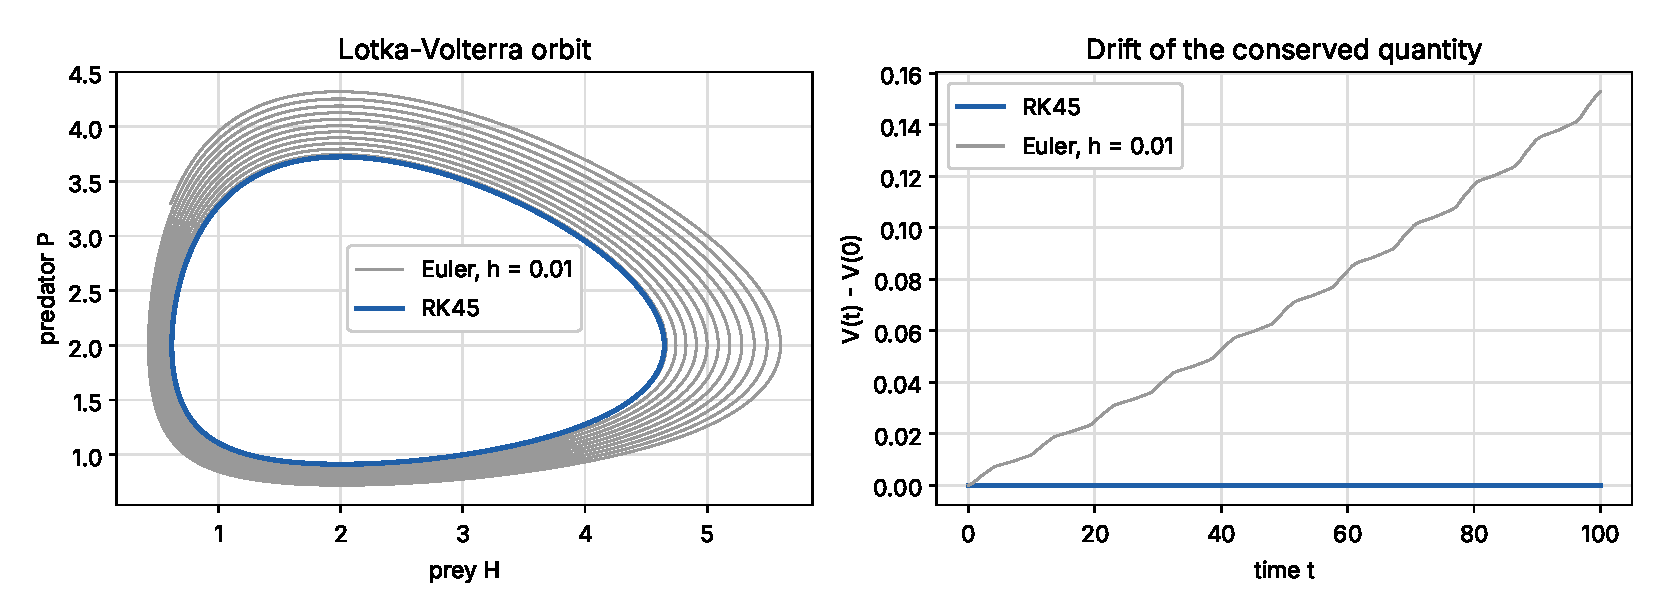
\includegraphics[width=0.9\linewidth]{rishi_solver_validation}
  \caption{Solver check on Lotka--Volterra. RK45 preserves the conserved quantity $V$ and
  closes the orbit; Euler ($h=0.01$) drifts and spirals outward. Only an accurate solver can
  distinguish a genuine limit cycle from a numerical artefact.}
  \label{fig:rishi_solver}
\end{figure}

\subsection{Reproduction of the analytic regimes}

Table~\ref{tab:rishi_regimes} reproduces each validation target of Section~\ref{sec:joel}
(3000-year burn-in throughout). Regime~D lies exactly on $K_H$: the residual oscillation there is
a slowly decaying transient (decay is only algebraic at a weak focus), not a cycle.

\begin{table}[htbp]
  \centering
  \caption{Simulated long-run behaviour for the regimes of Section~\ref{sec:joel}. Ranges are
  over 400 years after the burn-in; period and lynx lag are in years.}
  \label{tab:rishi_regimes}
  \begin{tabular}{clccccc}
    \toprule
    & $K$ & Eigenvalues & $H$ range & $P$ range & Period & Lag \\
    \midrule
    A & 25  & $-1.5,\ -0.073$ ($E_1$) & $25.0$         & $0$              & -- & -- \\
    B & 60  & $-0.188\pm0.515i$ & $30.0$         & $11.25$          & -- & -- \\
    C & 85  & $-0.022\pm0.623i$ & $30.0$         & $14.56$          & -- & -- \\
    D & 90  & $\pm0.632i$       & $[28.5,31.6]$  & $[14.51,15.49]$  & 9.94  & 2.50 \\
    E & 95  & $+0.020\pm0.640i$ & $[15.8,50.9]$  & $[9.81,20.75]$   & 10.25 & 2.81 \\
    F & 150 & $+0.150\pm0.676i$ & $[1.1,134.3]$  & $[1.69,41.16]$   & 13.91 & 4.52 \\
    \bottomrule
  \end{tabular}
\end{table}

Figure~\ref{fig:rishi_regimes} shows four of these regimes. Below the threshold (B, C) the
predator nullcline meets the prey hump to the right of its peak and trajectories spiral into
$E^*$; at $K=85$ the trace is only $-0.044$, so the decay takes centuries. Above the threshold
(E, F) the intersection lies left of the peak, $E^*$ repels, and the orbit settles onto a
sustained cycle that circulates counter-clockwise, with lynx peaks lagging hare peaks.

\begin{figure}[htbp]
  \centering
  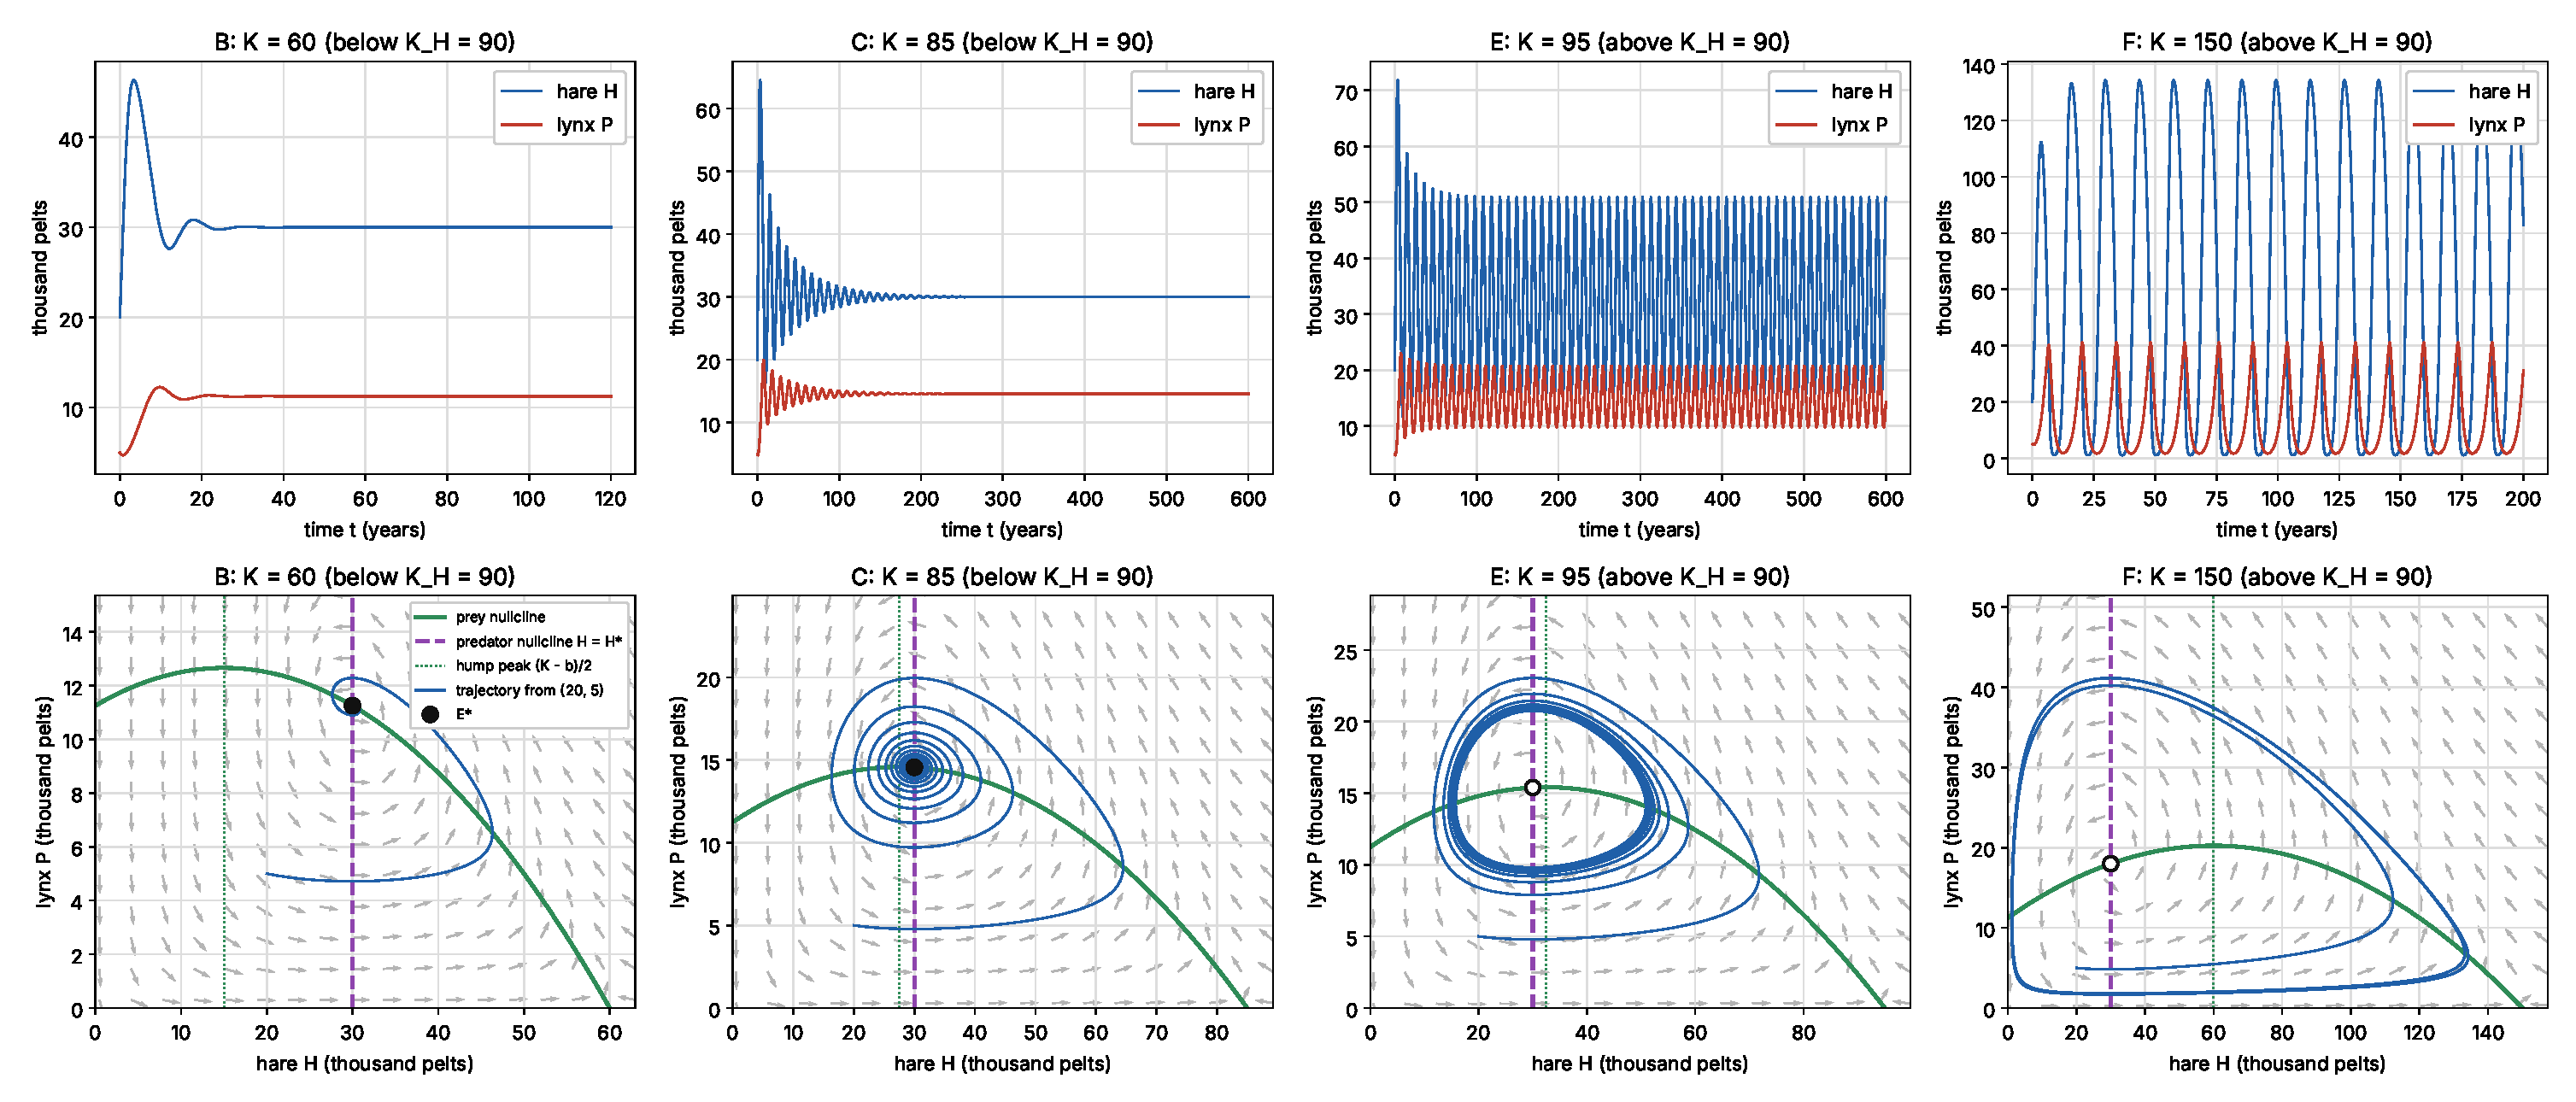
\includegraphics[width=\linewidth]{rishi_regimes}
  \caption{Time series (top) and phase portraits (bottom) from $(20,5)$ for $K=60,85$ (below
  $K_H=90$) and $K=95,150$ (above). Green: prey nullcline; dashed purple: predator nullcline
  $H=H^*$; dotted: hump peak $(K-b)/2$. Filled/open circle: stable/unstable $E^*$. Oscillations
  decay below $K_H$ and persist above it.}
  \label{fig:rishi_regimes}
\end{figure}

\subsection{The limit cycle attracts}

For Lotka--Volterra every initial condition lies on its own closed orbit. At $K=150$ we start one
trajectory beside the unstable equilibrium and one far outside the cycle
(Figure~\ref{fig:rishi_cycle}). The first spirals outward, the second inward, and their successive
hare maxima converge to the same value, $134.277$. The cycle is therefore orbitally stable,
in agreement with the uniqueness result cited in Section~\ref{sec:joel}~\cite{cheng1981}.

\begin{figure}[htbp]
  \centering
  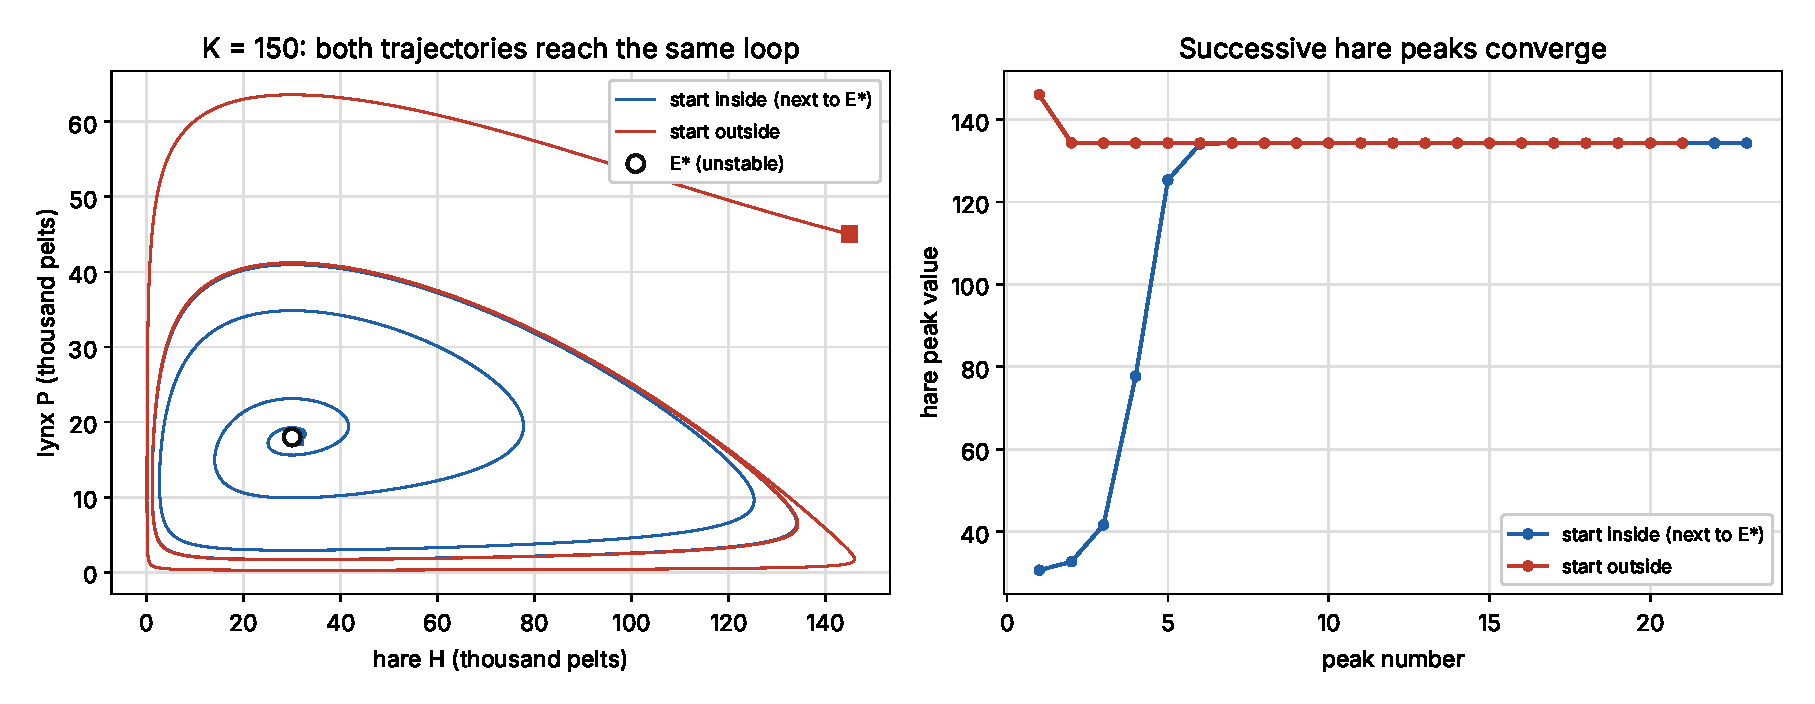
\includegraphics[width=0.9\linewidth]{rishi_limit_cycle}
  \caption{At $K=150$, trajectories started inside and outside the cycle converge onto the same
  closed orbit (left); their successive hare maxima approach a common value (right).}
  \label{fig:rishi_cycle}
\end{figure}

\subsection{Bifurcation in $K$}

Root-finding on the numerically evaluated trace of $J(E^*)$ places the sign change at
$K=90.0000000000$, in agreement with $K_H=b+2H^*$ and Figure~\ref{fig:trace-det}; there the
eigenvalues are $\pm0.632i=\pm i\omega_0$, and they become complex (node to focus) at $K\approx42.6$.

The numerical bifurcation diagram (Figure~\ref{fig:rishi_bif}) records the post-transient maximum
and minimum for 113 values of $K$ between 32 and 200. For $K<89$ the two coincide (largest
spread $5\times10^{-5}$): the solution settles on $E^*$. At $K_H$ the branches separate continuously
from the equilibrium and the cycle grows with $K$. Just above the threshold its half-amplitude
follows $A\approx7.8\sqrt{K-K_H}$, with fitted log--log slope $0.507$ for $0.5\le K-K_H\le8$
(Figure~\ref{fig:rishi_amp}), and the period approaches $T_0=9.93$ years ($9.97$ years at
$K-K_H=0.5$). This square-root growth from zero amplitude is the signature of a supercritical
Hopf bifurcation, consistent with the negative first Lyapunov coefficient of
Section~\ref{sec:joel}. As $K$ increases further the cycle minima approach zero: at $K=200$ the
hare minimum is $0.12$ thousand pelts, the paradox of enrichment~\cite{rosenzweig1971}.

\begin{figure}[htbp]
  \centering
  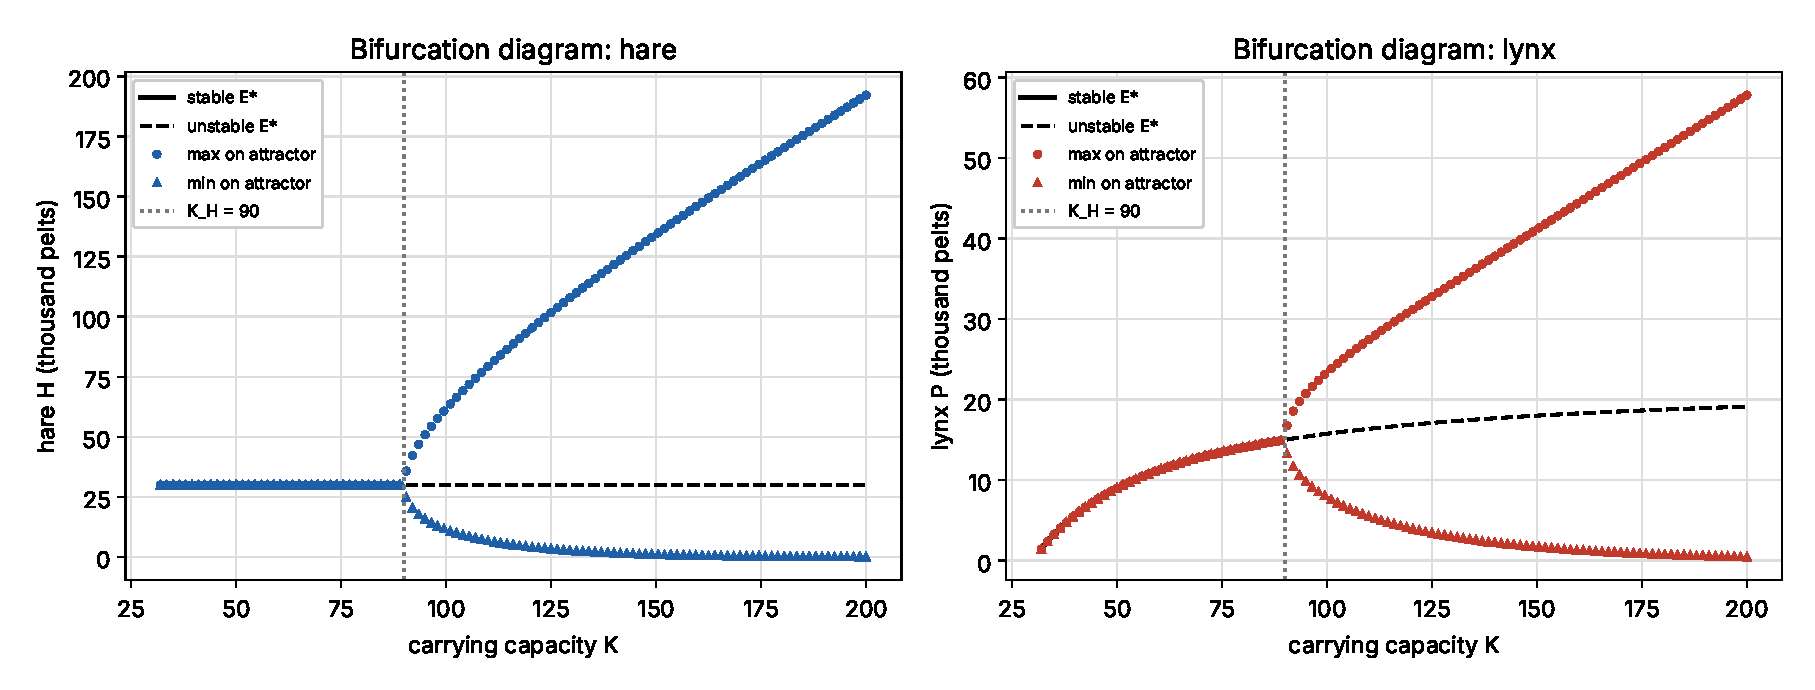
\includegraphics[width=0.9\linewidth]{rishi_bifurcation}
  \caption{Numerical bifurcation diagram: maximum and minimum of $H$ (left) and $P$ (right) after
  the burn-in, against $K$. Solid/dashed black: stable/unstable $E^*$. A cycle is born at
  $K_H=90$ with zero amplitude and its minima approach zero as $K$ grows.}
  \label{fig:rishi_bif}
\end{figure}

\begin{figure}[htbp]
  \centering
  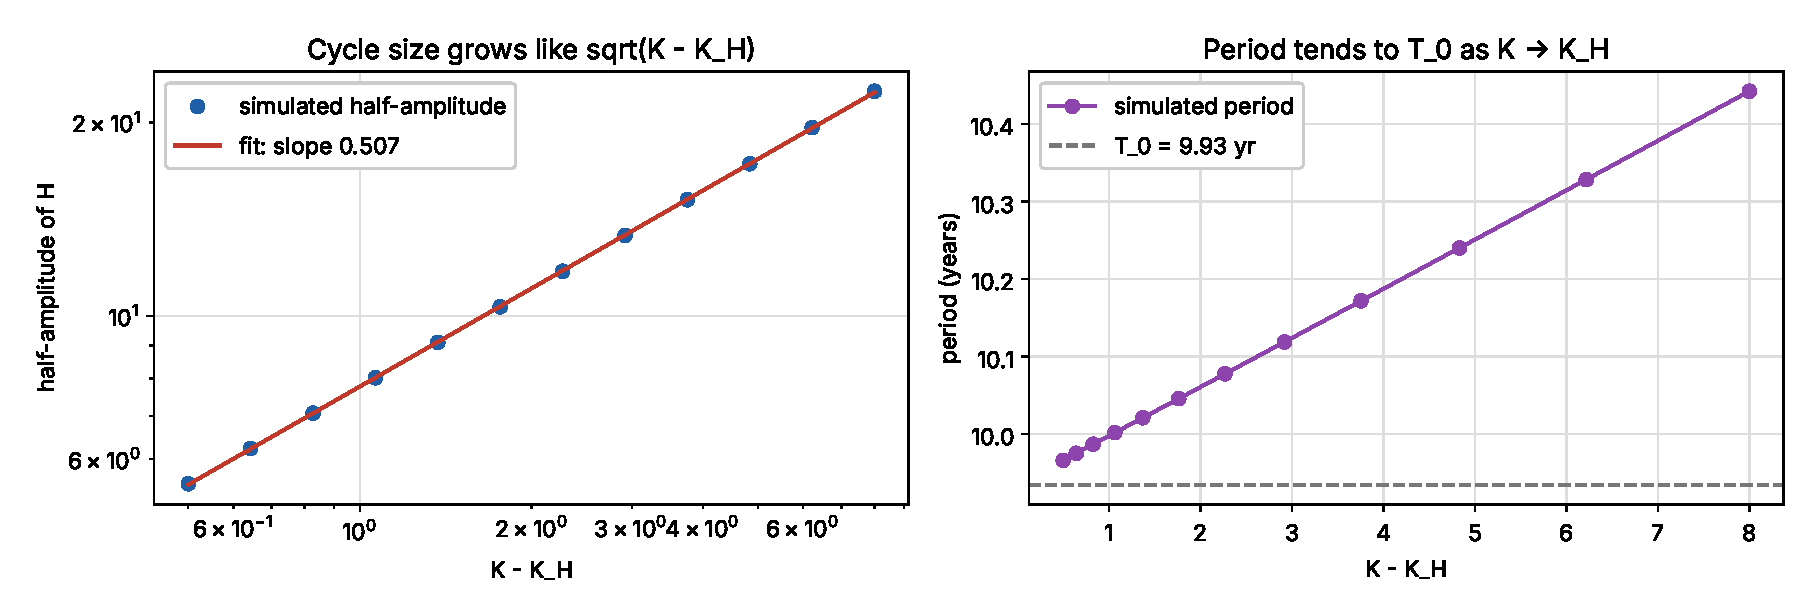
\includegraphics[width=0.9\linewidth]{rishi_amplitude_period}
  \caption{Left: half-amplitude of $H$ against $K-K_H$ on log--log axes, with slope $0.507$
  (supercritical prediction $1/2$). Right: cycle period, tending to $T_0=2\pi/\omega_0$.}
  \label{fig:rishi_amp}
\end{figure}

\subsection{Scope}

These simulations use illustrative, unfitted parameters and provide numerical evidence for one
parameter set, not proofs. Near $K_H$ the results depend on the burn-in length, which is why it
is lengthened there. Whether the historical hare--lynx series lies above or below the threshold
depends on $\sigma=K/K_H$ at the fitted parameters and is addressed in the fitting sections.
   (standalone build: rishi_main.tex)
%  Needs: amsmath, amssymb, booktabs, graphicx (PDF companions are used under pdflatex)
%  Figures: graphs/rishi_*.{eps,pdf}
%  Regenerate: python scripts/rishi_simulations.py   (numbers: results/simulations/)
%              python scripts/rishi_historical_placement.py   (results/simulations/historical/)
%  Code: src/lynx_hare/simulation.py, src/lynx_hare/simulation_plots.py,
%        notebooks/rishi_simulations.ipynb
% =====================================================================

\section{Numerical Simulations}\label{sec:rishi}

Section~\ref{sec:joel} locates the Hopf threshold $K_H=b+2H^*$ analytically. Linearisation is,
however, a local statement about the equilibrium at a single parameter value. This section tests
those predictions numerically and measures what linear analysis cannot give: the long-run
behaviour away from $E^*$, the size and period of the cycle, and the shape of the bifurcation.
Every trajectory is computed with the group's shared right-hand side of~\eqref{eq:rm}.

\subsection{Method}

\paragraph{Parameters.} We use the illustrative, unfitted values of Section~\ref{sec:joel}:
$r=1.5$, $a=4$, $b=30$, $e=0.4$, $m=0.8$ ($H,P$ in thousands of pelts, $t$ in years), for which
$H^*=30$, $K_H=90$ and $T_0=2\pi/\omega_0\approx 9.94$ years. The carrying capacity $K$ is varied.

\paragraph{Solver.} Equations~\eqref{eq:rm} are integrated with the adaptive Dormand--Prince
Runge--Kutta pair (RK45) in \texttt{scipy.integrate.solve\_ivp}~\cite{dormand1980,scipysolve}.
At each step a fourth- and a fifth-order estimate are formed from the same seven slope
evaluations; their difference estimates the local error, and the step is rejected and reduced
whenever this exceeds $\texttt{rtol}\,|y|+\texttt{atol}$. The project uses two settings of this
solver for two different jobs. Fitting and the 1900--1920 forecasts of the historical sections use
\texttt{model.solve} with $\texttt{rtol}=10^{-8}$, $\texttt{atol}=10^{-10}$ and a maximum step of
$0.1$ years, identical for both fitting methods. The long-run simulations in this section run for
thousands of years, so they use tighter tolerances, $\texttt{rtol}=10^{-10}$ and
$\texttt{atol}=10^{-12}$, without a step cap. Both call the same shared right-hand side. The
illustrative runs start from $(H_0,P_0)=(20,5)$; all values are in
\texttt{configs/simulations.json}.

\paragraph{Long-run behaviour.} To describe the attractor we integrate for a burn-in period
$T_{\mathrm{burn}}$, discard it, and record the next 300--400 years. On the recorded window we
report the range of $H$ and $P$; if $H$ still oscillates, the period is the mean interval between
successive hare maxima and the lag is the mean delay from a hare maximum to the next lynx
maximum. We take $T_{\mathrm{burn}}=3000$ years, increased to $20{,}000$ years when
$|K-K_H|<1$, where the equilibrium is a weak focus and transients decay very slowly.

\subsection{Solver accuracy}

The classical Lotka--Volterra system $\dot H=\alpha H-\beta HP$, $\dot P=\delta HP-\gamma P$
conserves $V=\delta H-\gamma\ln H+\beta P-\alpha\ln P$, so any drift in $V$ along a computed
orbit is numerical error. Over 100 time units RK45 keeps $|V(t)-V(0)|$ below $4\times10^{-10}$,
whereas explicit Euler with step $h=0.01$ drifts by $0.15$ and its orbit spirals outward
(Figure~\ref{fig:rishi_solver}), creating oscillatory growth the model does not have. For
Rosenzweig--MacArthur at $K=150$, tightening both tolerances a hundredfold changes the
solution by a relative $8\times10^{-10}$, and all states remain positive, as Lemma~\ref{lem:bounded}
requires.

\begin{figure}[htbp]
  \centering
  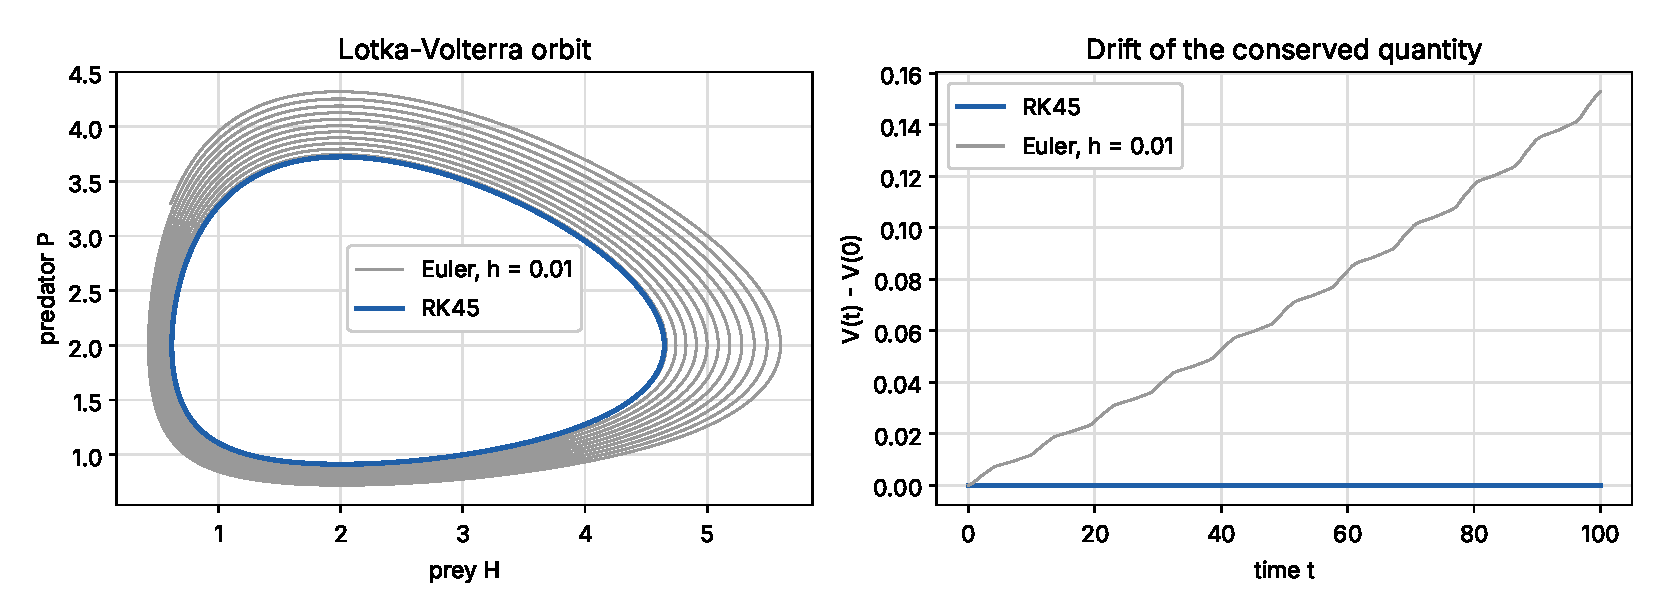
\includegraphics[width=0.9\linewidth]{rishi_solver_validation}
  \caption{Solver check on Lotka--Volterra. RK45 preserves the conserved quantity $V$ and
  closes the orbit; Euler ($h=0.01$) drifts and spirals outward. Only an accurate solver can
  distinguish a genuine limit cycle from a numerical artefact.}
  \label{fig:rishi_solver}
\end{figure}

\subsection{Reproduction of the analytic regimes}

Table~\ref{tab:rishi_regimes} reproduces each validation target of Section~\ref{sec:joel}
(3000-year burn-in throughout). Regime~D lies exactly on $K_H$: the residual oscillation there is
a slowly decaying transient (decay is only algebraic at a weak focus), not a cycle.

\begin{table}[htbp]
  \centering
  \caption{Simulated long-run behaviour for the regimes of Section~\ref{sec:joel}. Ranges are
  over 400 years after the burn-in; period and lynx lag are in years.}
  \label{tab:rishi_regimes}
  \begin{tabular}{clccccc}
    \toprule
    & $K$ & Eigenvalues & $H$ range & $P$ range & Period & Lag \\
    \midrule
    A & 25  & $-1.5,\ -0.073$ ($E_1$) & $25.0$         & $0$              & -- & -- \\
    B & 60  & $-0.188\pm0.515i$ & $30.0$         & $11.25$          & -- & -- \\
    C & 85  & $-0.022\pm0.623i$ & $30.0$         & $14.56$          & -- & -- \\
    D & 90  & $\pm0.632i$       & $[28.5,31.6]$  & $[14.51,15.49]$  & 9.94  & 2.50 \\
    E & 95  & $+0.020\pm0.640i$ & $[15.8,50.9]$  & $[9.81,20.75]$   & 10.25 & 2.81 \\
    F & 150 & $+0.150\pm0.676i$ & $[1.1,134.3]$  & $[1.69,41.16]$   & 13.91 & 4.52 \\
    \bottomrule
  \end{tabular}
\end{table}

Figure~\ref{fig:rishi_regimes} shows four of these regimes. Below the threshold (B, C) the
predator nullcline meets the prey hump to the right of its peak and trajectories spiral into
$E^*$; at $K=85$ the trace is only $-0.044$, so the decay takes centuries. Above the threshold
(E, F) the intersection lies left of the peak, $E^*$ repels, and the orbit settles onto a
sustained cycle that circulates counter-clockwise, with lynx peaks lagging hare peaks.

\begin{figure}[htbp]
  \centering
  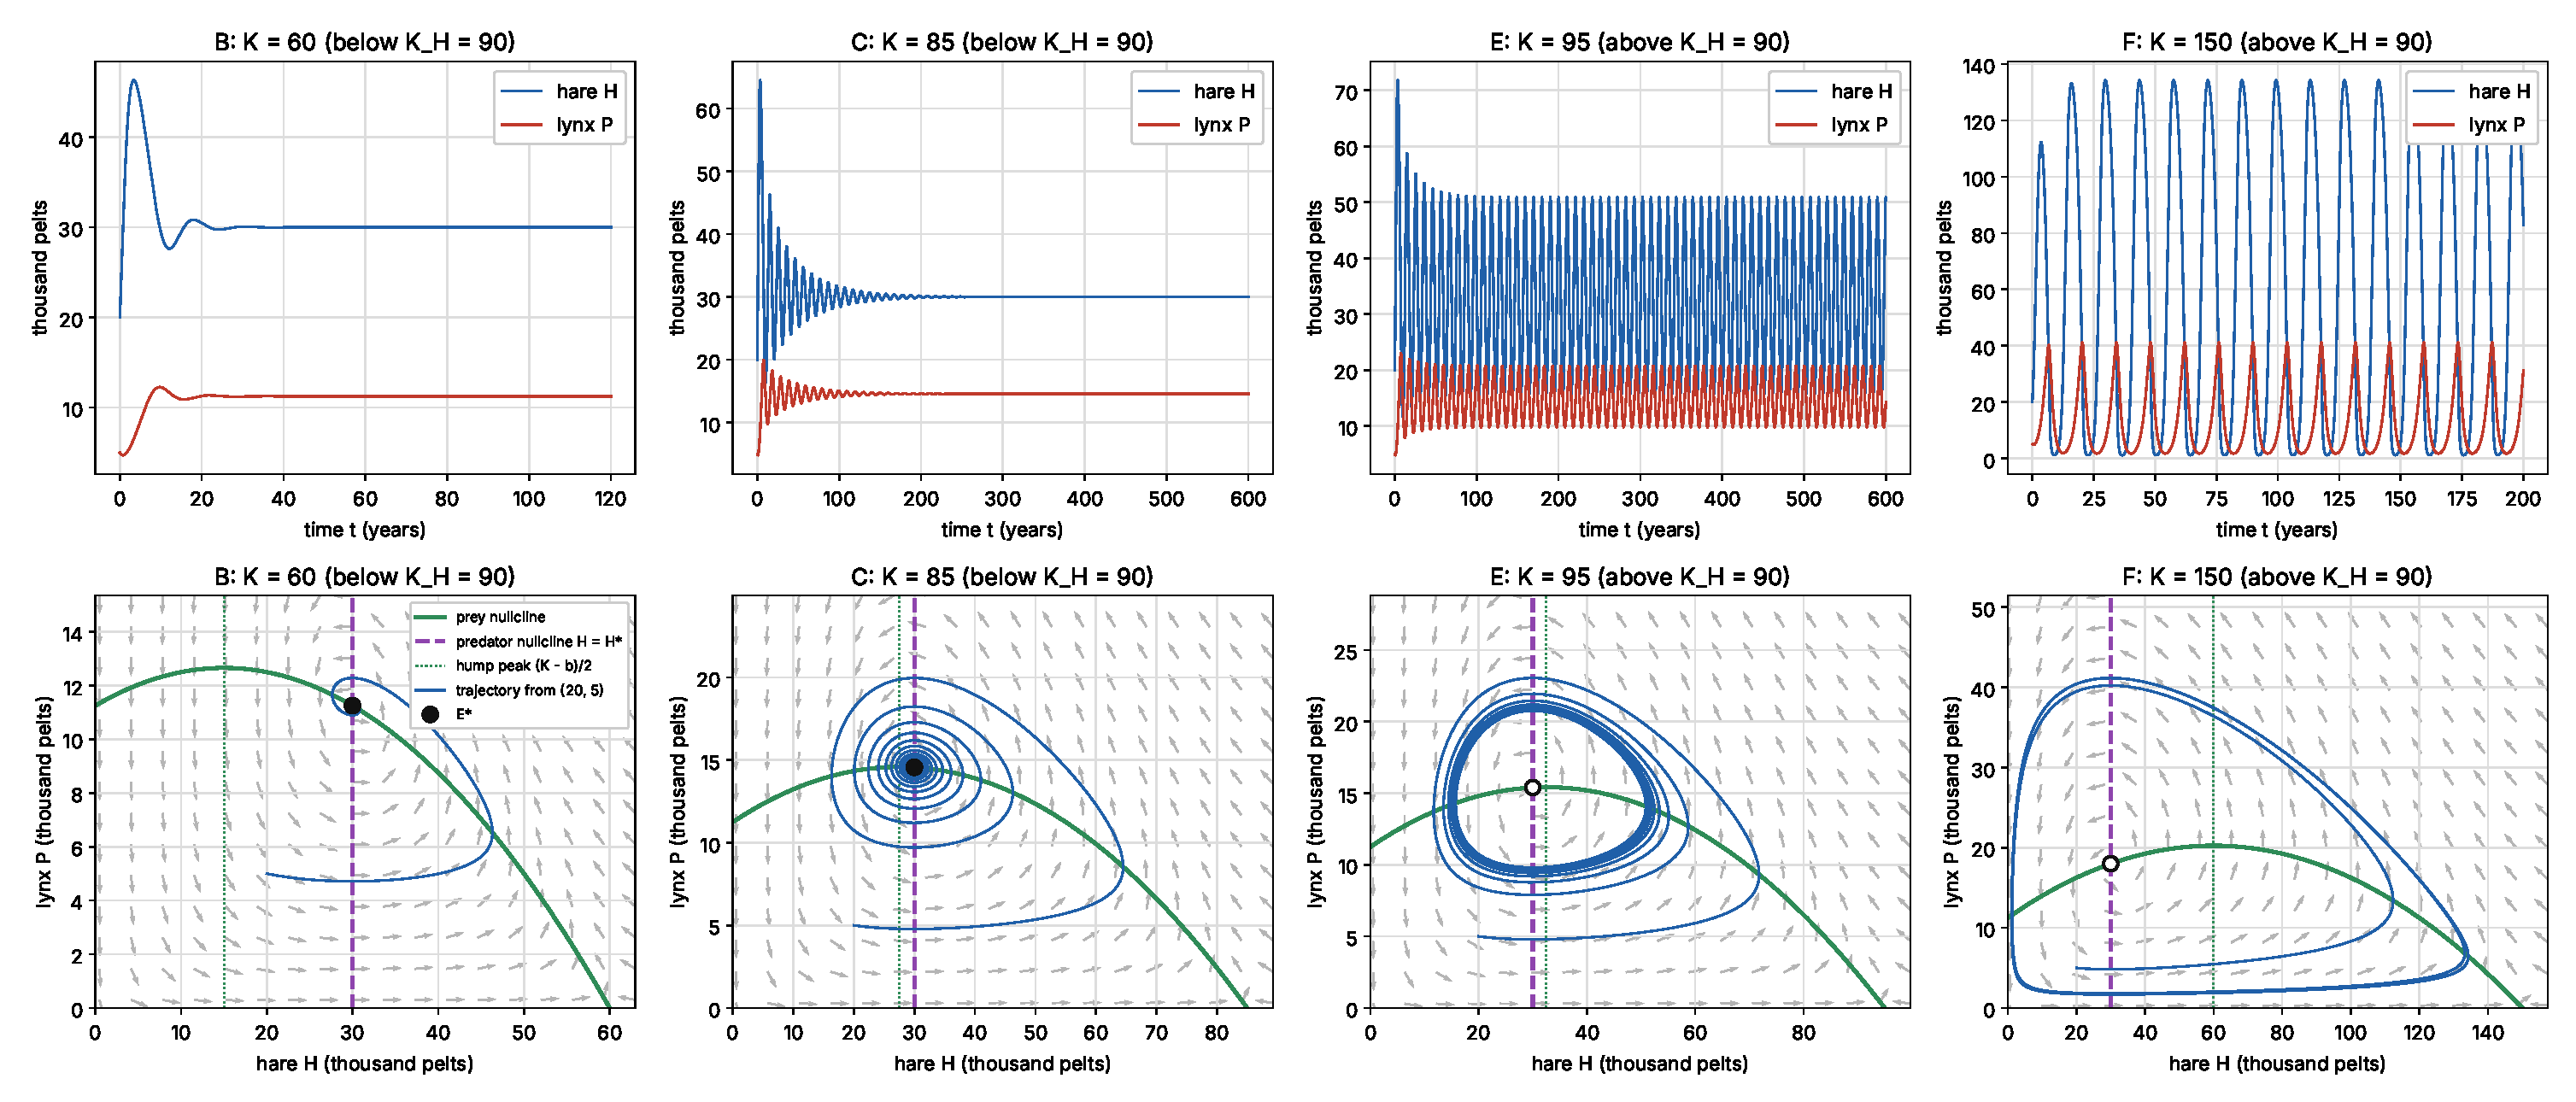
\includegraphics[width=\linewidth]{rishi_regimes}
  \caption{Time series (top) and phase portraits (bottom) from $(20,5)$ for $K=60,85$ (below
  $K_H=90$) and $K=95,150$ (above). Green: prey nullcline; dashed purple: predator nullcline
  $H=H^*$; dotted: hump peak $(K-b)/2$. Filled/open circle: stable/unstable $E^*$. Oscillations
  decay below $K_H$ and persist above it.}
  \label{fig:rishi_regimes}
\end{figure}

\subsection{The limit cycle attracts}

For Lotka--Volterra every initial condition lies on its own closed orbit. At $K=150$ we start one
trajectory beside the unstable equilibrium and one far outside the cycle
(Figure~\ref{fig:rishi_cycle}). The first spirals outward, the second inward, and their successive
hare maxima converge to the same value, $134.277$. The cycle is therefore orbitally stable,
in agreement with the uniqueness result cited in Section~\ref{sec:joel}~\cite{cheng1981}.

\begin{figure}[htbp]
  \centering
  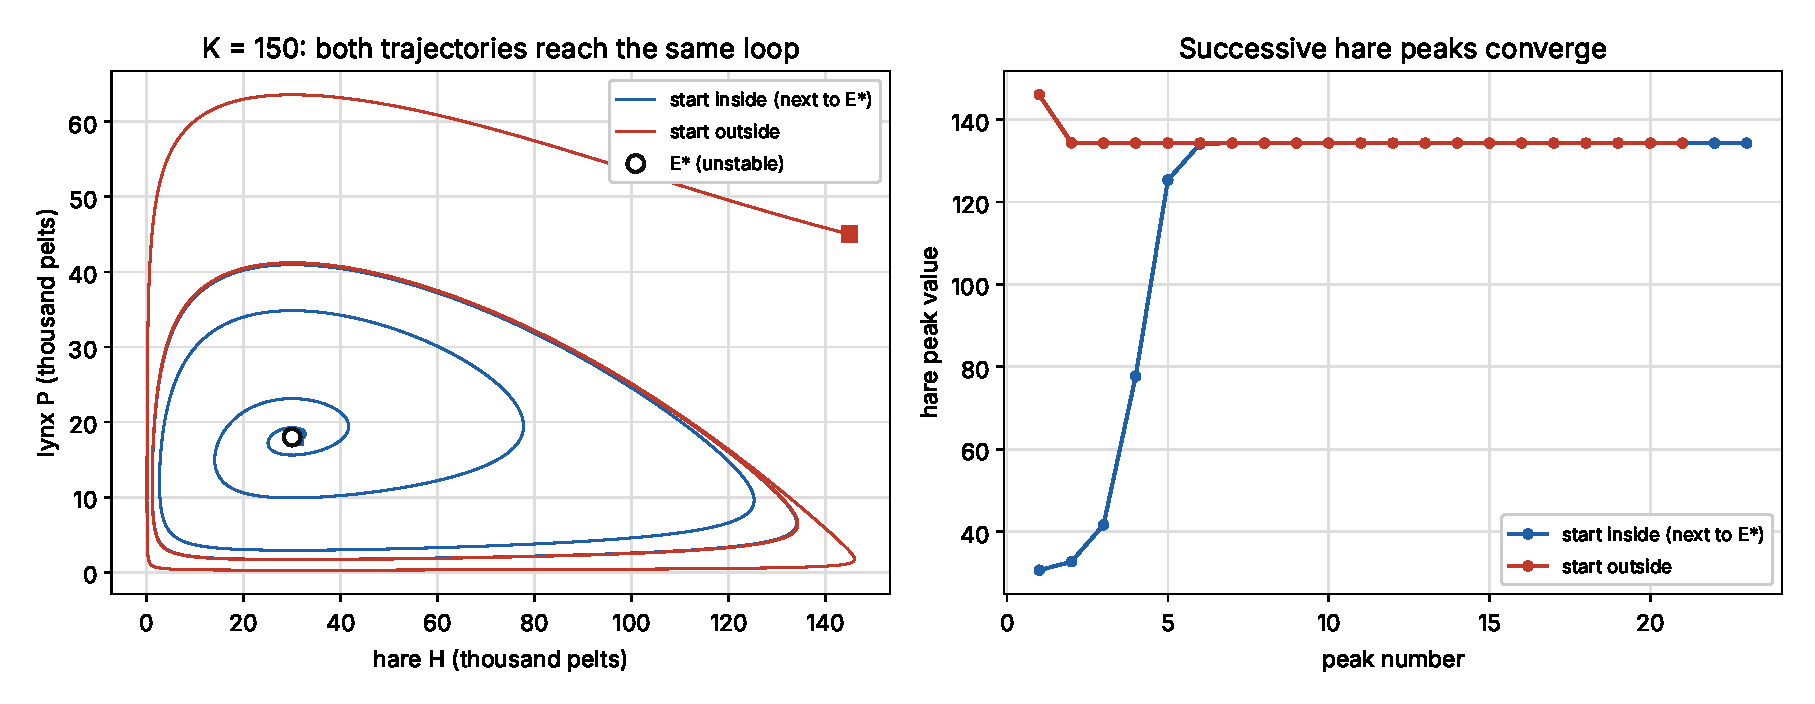
\includegraphics[width=0.9\linewidth]{rishi_limit_cycle}
  \caption{At $K=150$, trajectories started inside and outside the cycle converge onto the same
  closed orbit (left); their successive hare maxima approach a common value (right).}
  \label{fig:rishi_cycle}
\end{figure}

\subsection{Bifurcation in $K$}

Root-finding on the numerically evaluated trace of $J(E^*)$ places the sign change at
$K=90.0000000000$, in agreement with $K_H=b+2H^*$ and Figure~\ref{fig:trace-det}; there the
eigenvalues are $\pm0.632i=\pm i\omega_0$, and they become complex (node to focus) at $K\approx42.6$.

The numerical bifurcation diagram (Figure~\ref{fig:rishi_bif}) records the post-transient maximum
and minimum for 113 values of $K$ between 32 and 200. For $K<89$ the two coincide (largest
spread $5\times10^{-5}$): the solution settles on $E^*$. At $K_H$ the branches separate continuously
from the equilibrium and the cycle grows with $K$. Just above the threshold its half-amplitude
follows $A\approx7.8\sqrt{K-K_H}$, with fitted log--log slope $0.507$ for $0.5\le K-K_H\le8$
(Figure~\ref{fig:rishi_amp}), and the period approaches $T_0=9.93$ years ($9.97$ years at
$K-K_H=0.5$). This square-root growth from zero amplitude is the signature of a supercritical
Hopf bifurcation, consistent with the negative first Lyapunov coefficient of
Section~\ref{sec:joel}. As $K$ increases further the cycle minima approach zero: at $K=200$ the
hare minimum is $0.12$ thousand pelts, the paradox of enrichment~\cite{rosenzweig1971}.

\begin{figure}[htbp]
  \centering
  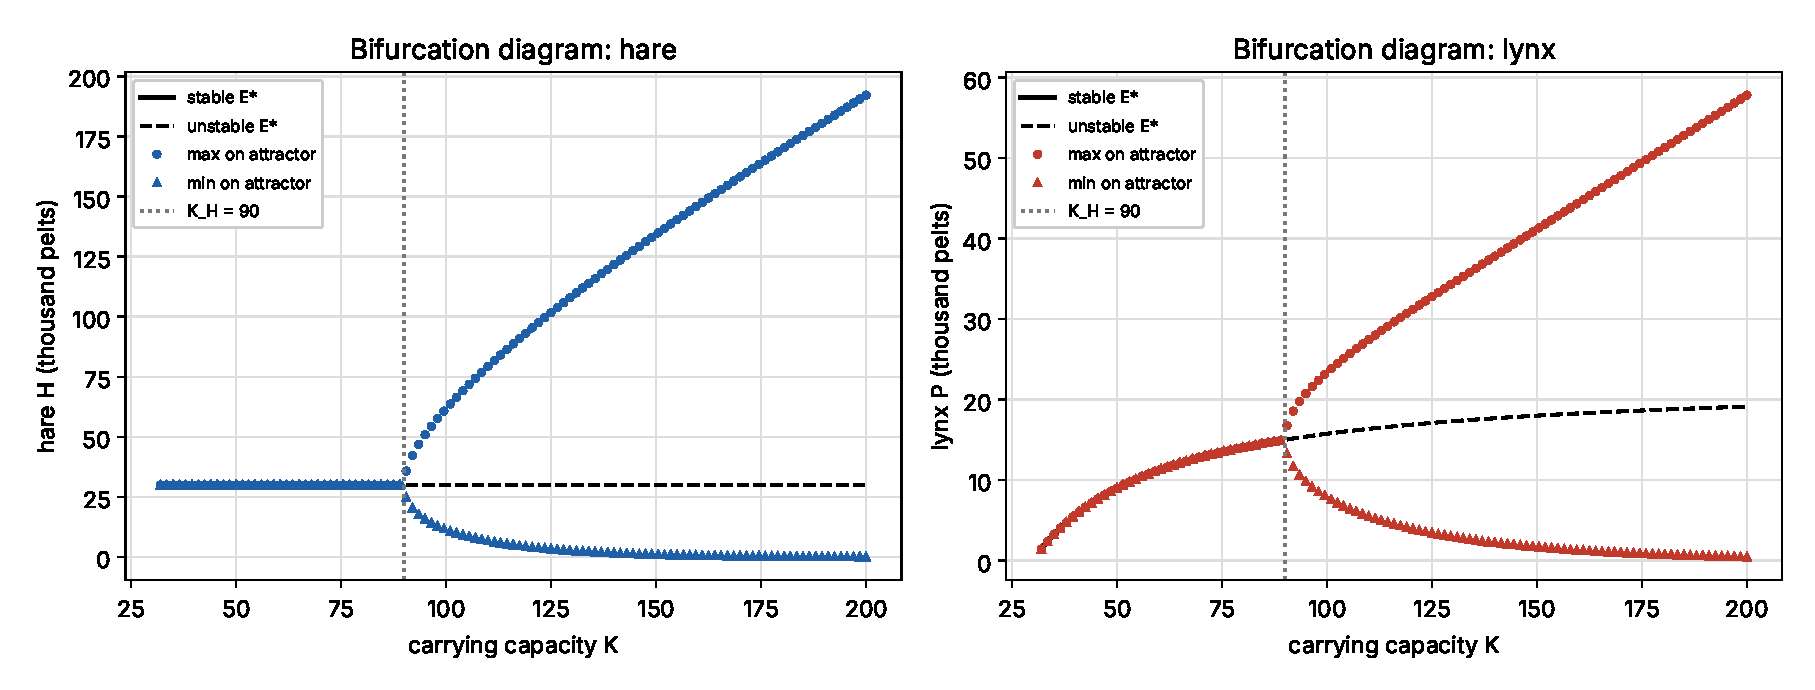
\includegraphics[width=0.9\linewidth]{rishi_bifurcation}
  \caption{Numerical bifurcation diagram: maximum and minimum of $H$ (left) and $P$ (right) after
  the burn-in, against $K$. Solid/dashed black: stable/unstable $E^*$. A cycle is born at
  $K_H=90$ with zero amplitude and its minima approach zero as $K$ grows.}
  \label{fig:rishi_bif}
\end{figure}

\begin{figure}[htbp]
  \centering
  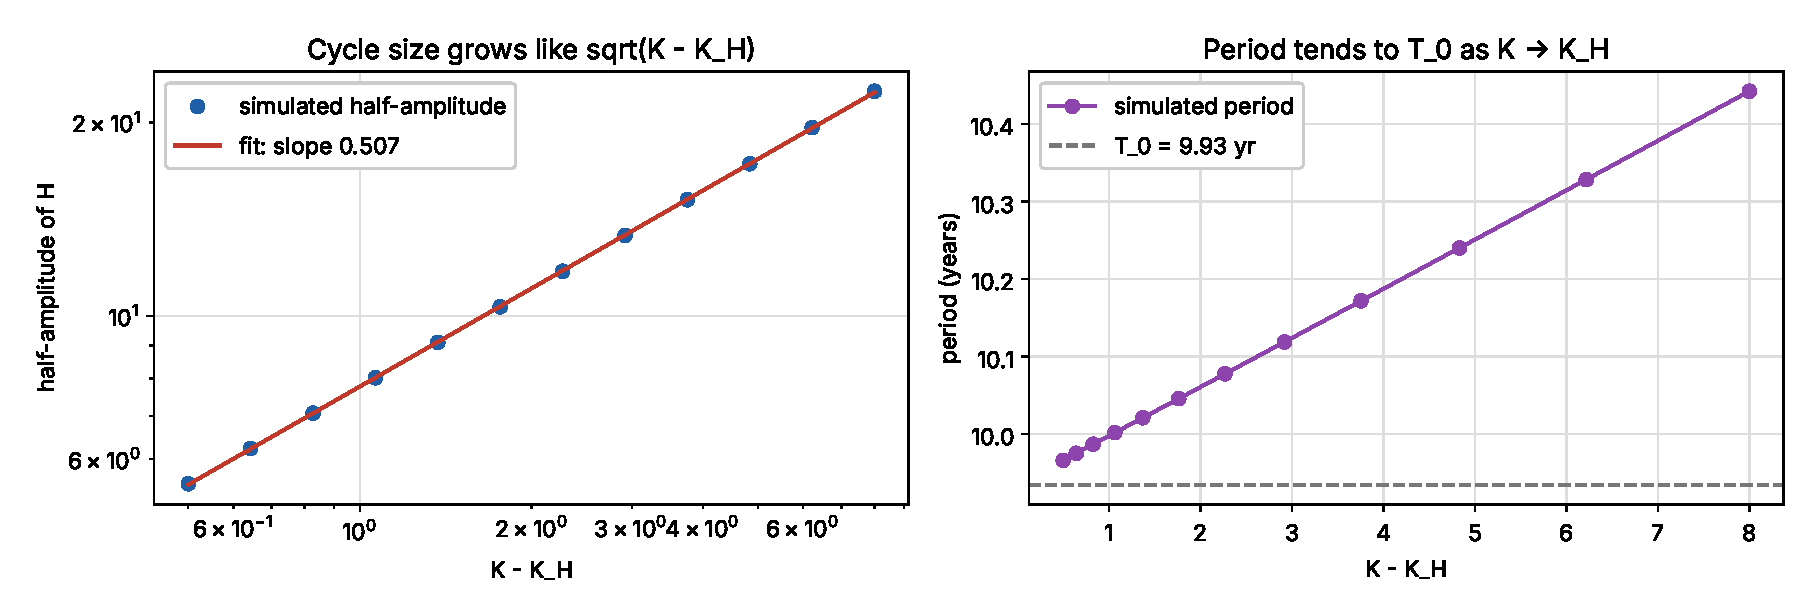
\includegraphics[width=0.9\linewidth]{rishi_amplitude_period}
  \caption{Left: half-amplitude of $H$ against $K-K_H$ on log--log axes, with slope $0.507$
  (supercritical prediction $1/2$). Right: cycle period, tending to $T_0=2\pi/\omega_0$.}
  \label{fig:rishi_amp}
\end{figure}

\subsection{Scope}

These simulations use illustrative, unfitted parameters and provide numerical evidence for one
parameter set, not proofs. Near $K_H$ the results depend on the burn-in length, which is why it
is lengthened there. Whether the historical hare--lynx series lies above or below the threshold
depends on $\sigma=K/K_H$ at the fitted parameters and is addressed in the fitting sections.
   (standalone build: rishi_main.tex)
%  Needs: amsmath, amssymb, booktabs, graphicx (PDF companions are used under pdflatex)
%  Figures: graphs/rishi_*.{eps,pdf}
%  Regenerate: python scripts/rishi_simulations.py   (numbers: results/simulations/)
%              python scripts/rishi_historical_placement.py   (results/simulations/historical/)
%  Code: src/lynx_hare/simulation.py, src/lynx_hare/simulation_plots.py,
%        notebooks/rishi_simulations.ipynb
% =====================================================================

\section{Numerical Simulations}\label{sec:rishi}

Section~\ref{sec:joel} locates the Hopf threshold $K_H=b+2H^*$ analytically. Linearisation is,
however, a local statement about the equilibrium at a single parameter value. This section tests
those predictions numerically and measures what linear analysis cannot give: the long-run
behaviour away from $E^*$, the size and period of the cycle, and the shape of the bifurcation.
Every trajectory is computed with the group's shared right-hand side of~\eqref{eq:rm}.

\subsection{Method}

\paragraph{Parameters.} We use the illustrative, unfitted values of Section~\ref{sec:joel}:
$r=1.5$, $a=4$, $b=30$, $e=0.4$, $m=0.8$ ($H,P$ in thousands of pelts, $t$ in years), for which
$H^*=30$, $K_H=90$ and $T_0=2\pi/\omega_0\approx 9.94$ years. The carrying capacity $K$ is varied.

\paragraph{Solver.} Equations~\eqref{eq:rm} are integrated with the adaptive Dormand--Prince
Runge--Kutta pair (RK45) in \texttt{scipy.integrate.solve\_ivp}~\cite{dormand1980,scipysolve}.
At each step a fourth- and a fifth-order estimate are formed from the same seven slope
evaluations; their difference estimates the local error, and the step is rejected and reduced
whenever this exceeds $\texttt{rtol}\,|y|+\texttt{atol}$. The project uses two settings of this
solver for two different jobs. Fitting and the 1900--1920 forecasts of the historical sections use
\texttt{model.solve} with $\texttt{rtol}=10^{-8}$, $\texttt{atol}=10^{-10}$ and a maximum step of
$0.1$ years, identical for both fitting methods. The long-run simulations in this section run for
thousands of years, so they use tighter tolerances, $\texttt{rtol}=10^{-10}$ and
$\texttt{atol}=10^{-12}$, without a step cap. Both call the same shared right-hand side. The
illustrative runs start from $(H_0,P_0)=(20,5)$; all values are in
\texttt{configs/simulations.json}.

\paragraph{Long-run behaviour.} To describe the attractor we integrate for a burn-in period
$T_{\mathrm{burn}}$, discard it, and record the next 300--400 years. On the recorded window we
report the range of $H$ and $P$; if $H$ still oscillates, the period is the mean interval between
successive hare maxima and the lag is the mean delay from a hare maximum to the next lynx
maximum. We take $T_{\mathrm{burn}}=3000$ years, increased to $20{,}000$ years when
$|K-K_H|<1$, where the equilibrium is a weak focus and transients decay very slowly.

\subsection{Solver accuracy}

The classical Lotka--Volterra system $\dot H=\alpha H-\beta HP$, $\dot P=\delta HP-\gamma P$
conserves $V=\delta H-\gamma\ln H+\beta P-\alpha\ln P$, so any drift in $V$ along a computed
orbit is numerical error. Over 100 time units RK45 keeps $|V(t)-V(0)|$ below $4\times10^{-10}$,
whereas explicit Euler with step $h=0.01$ drifts by $0.15$ and its orbit spirals outward
(Figure~\ref{fig:rishi_solver}), creating oscillatory growth the model does not have. For
Rosenzweig--MacArthur at $K=150$, tightening both tolerances a hundredfold changes the
solution by a relative $8\times10^{-10}$, and all states remain positive, as Lemma~\ref{lem:bounded}
requires.

\begin{figure}[htbp]
  \centering
  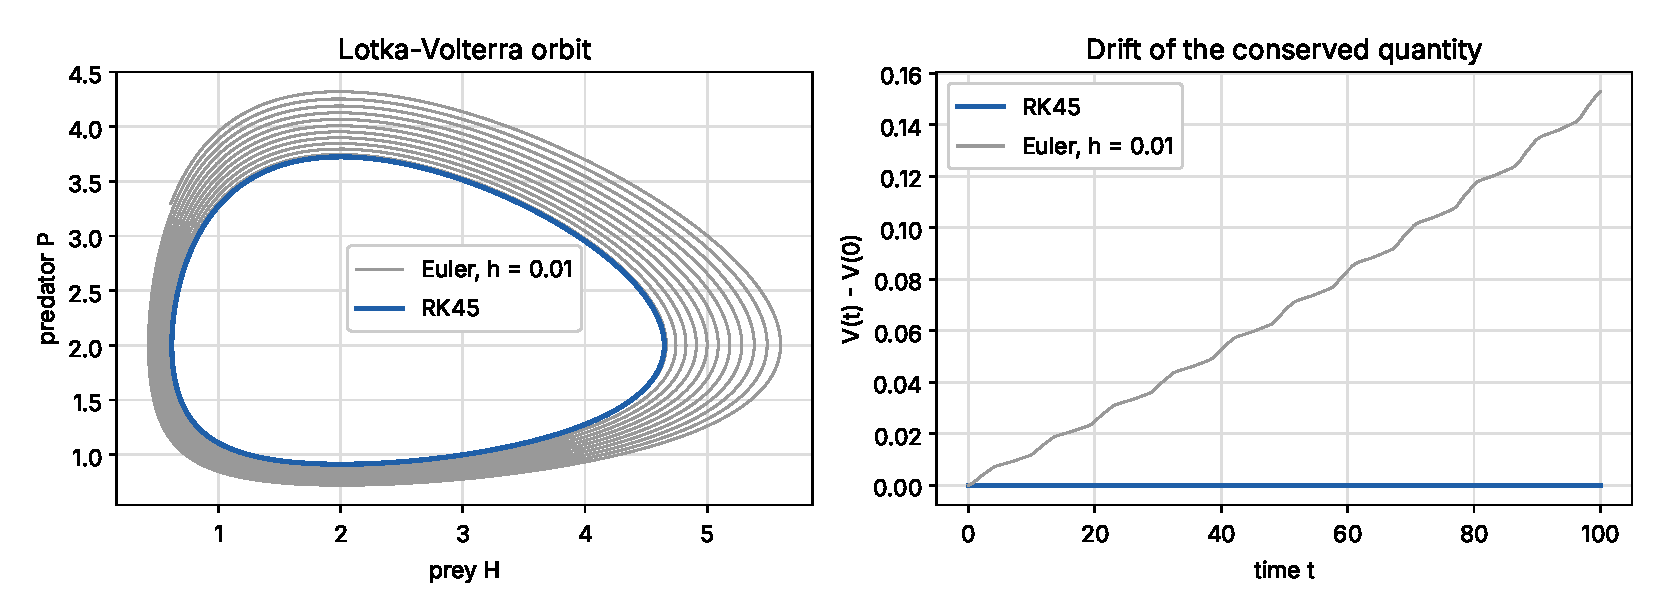
\includegraphics[width=0.9\linewidth]{rishi_solver_validation}
  \caption{Solver check on Lotka--Volterra. RK45 preserves the conserved quantity $V$ and
  closes the orbit; Euler ($h=0.01$) drifts and spirals outward. Only an accurate solver can
  distinguish a genuine limit cycle from a numerical artefact.}
  \label{fig:rishi_solver}
\end{figure}

\subsection{Reproduction of the analytic regimes}

Table~\ref{tab:rishi_regimes} reproduces each validation target of Section~\ref{sec:joel}
(3000-year burn-in throughout). Regime~D lies exactly on $K_H$: the residual oscillation there is
a slowly decaying transient (decay is only algebraic at a weak focus), not a cycle.

\begin{table}[htbp]
  \centering
  \caption{Simulated long-run behaviour for the regimes of Section~\ref{sec:joel}. Ranges are
  over 400 years after the burn-in; period and lynx lag are in years.}
  \label{tab:rishi_regimes}
  \begin{tabular}{clccccc}
    \toprule
    & $K$ & Eigenvalues & $H$ range & $P$ range & Period & Lag \\
    \midrule
    A & 25  & $-1.5,\ -0.073$ ($E_1$) & $25.0$         & $0$              & -- & -- \\
    B & 60  & $-0.188\pm0.515i$ & $30.0$         & $11.25$          & -- & -- \\
    C & 85  & $-0.022\pm0.623i$ & $30.0$         & $14.56$          & -- & -- \\
    D & 90  & $\pm0.632i$       & $[28.5,31.6]$  & $[14.51,15.49]$  & 9.94  & 2.50 \\
    E & 95  & $+0.020\pm0.640i$ & $[15.8,50.9]$  & $[9.81,20.75]$   & 10.25 & 2.81 \\
    F & 150 & $+0.150\pm0.676i$ & $[1.1,134.3]$  & $[1.69,41.16]$   & 13.91 & 4.52 \\
    \bottomrule
  \end{tabular}
\end{table}

Figure~\ref{fig:rishi_regimes} shows four of these regimes. Below the threshold (B, C) the
predator nullcline meets the prey hump to the right of its peak and trajectories spiral into
$E^*$; at $K=85$ the trace is only $-0.044$, so the decay takes centuries. Above the threshold
(E, F) the intersection lies left of the peak, $E^*$ repels, and the orbit settles onto a
sustained cycle that circulates counter-clockwise, with lynx peaks lagging hare peaks.

\begin{figure}[htbp]
  \centering
  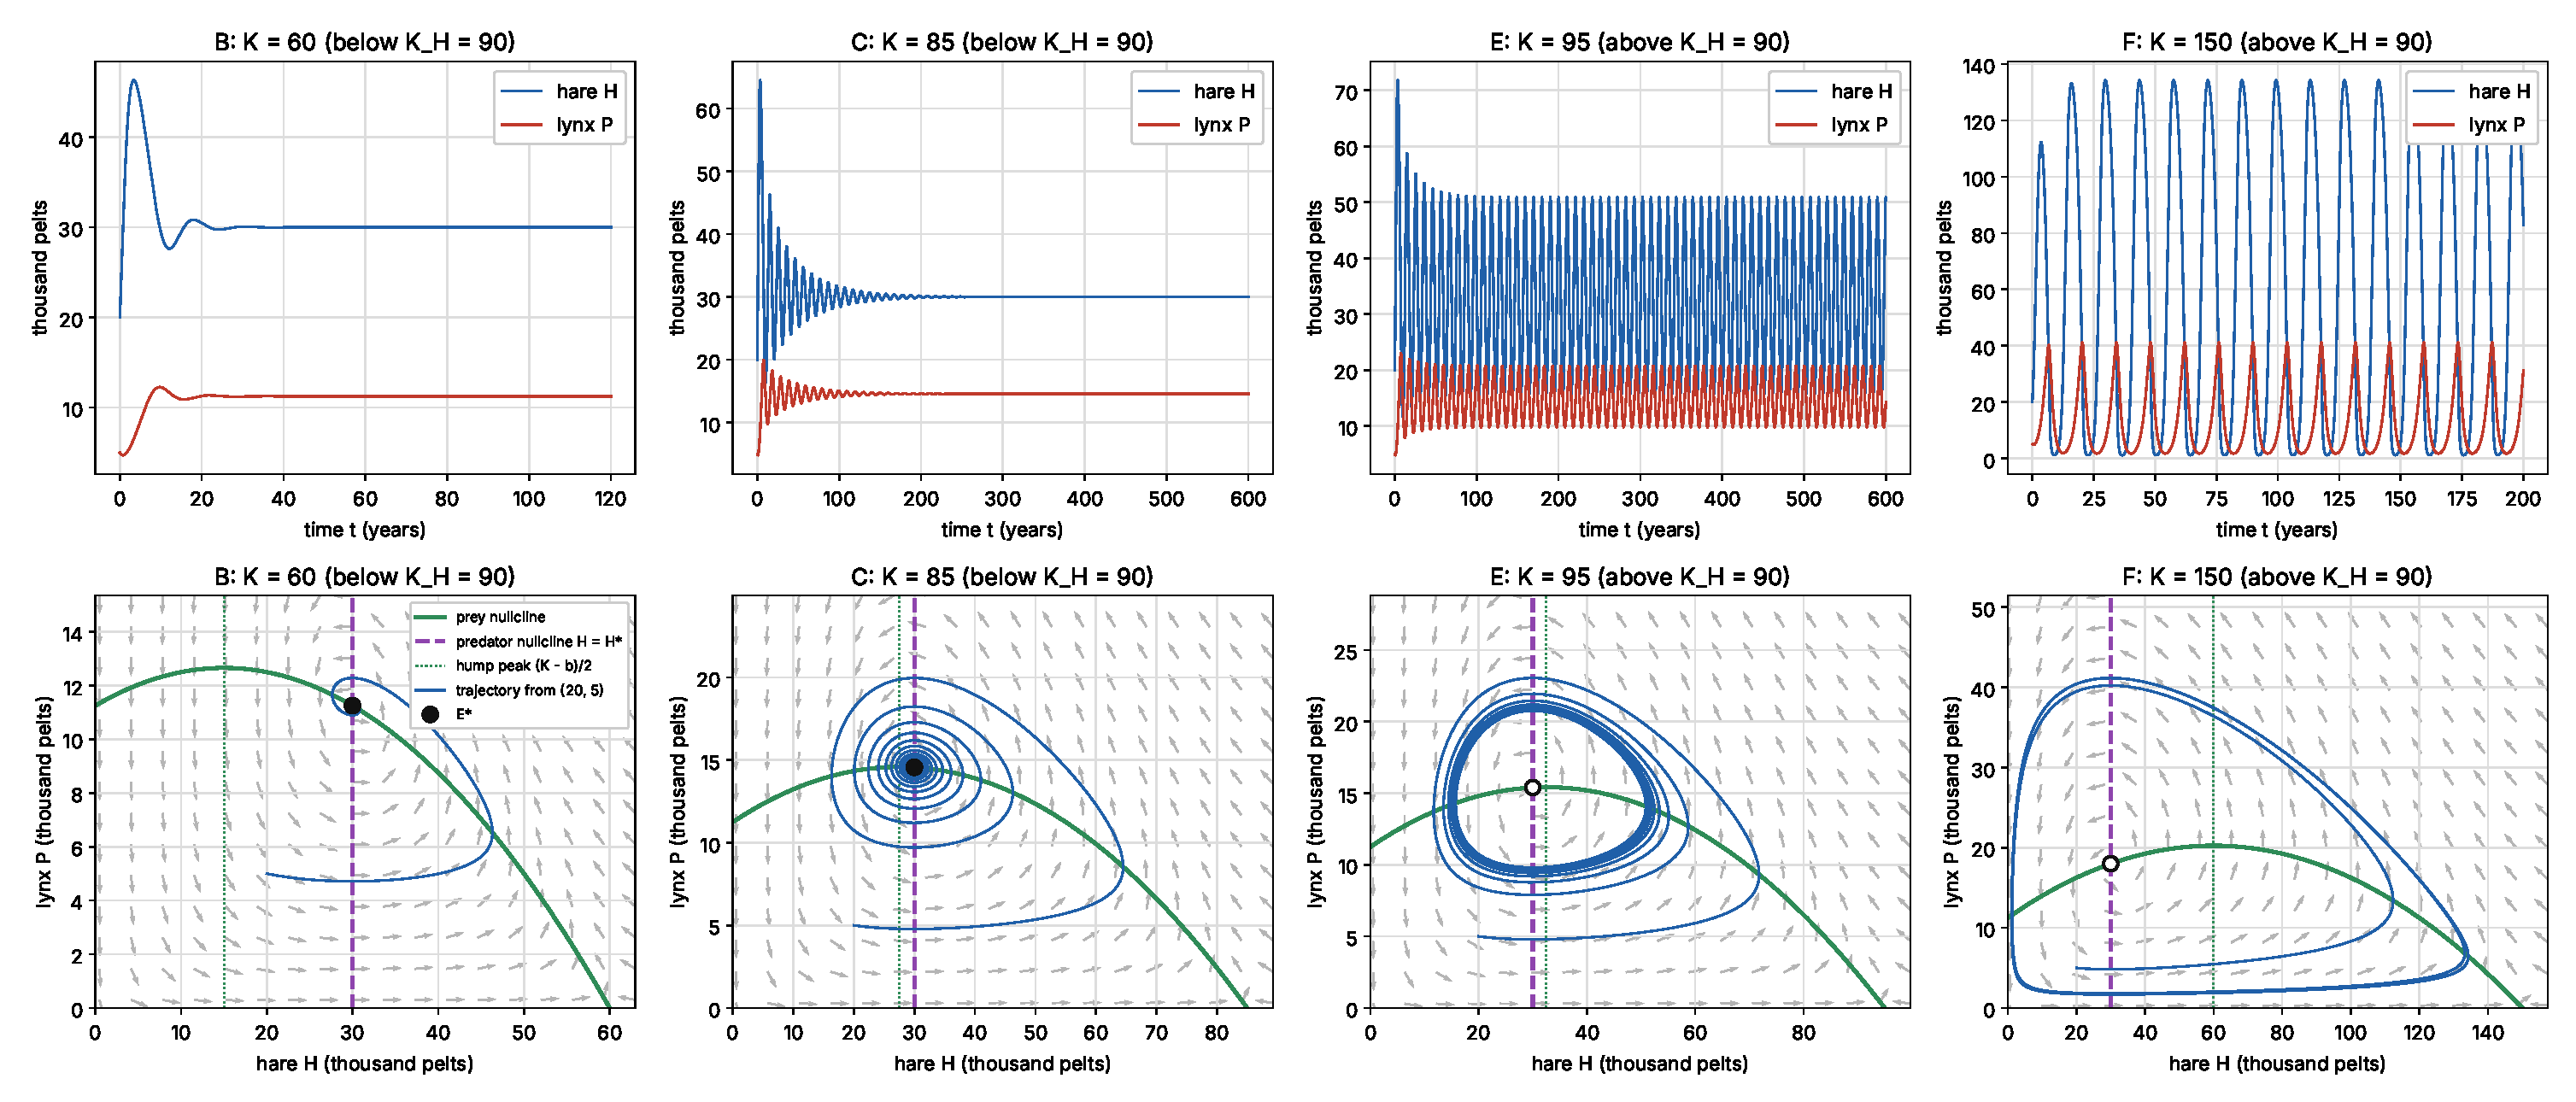
\includegraphics[width=\linewidth]{rishi_regimes}
  \caption{Time series (top) and phase portraits (bottom) from $(20,5)$ for $K=60,85$ (below
  $K_H=90$) and $K=95,150$ (above). Green: prey nullcline; dashed purple: predator nullcline
  $H=H^*$; dotted: hump peak $(K-b)/2$. Filled/open circle: stable/unstable $E^*$. Oscillations
  decay below $K_H$ and persist above it.}
  \label{fig:rishi_regimes}
\end{figure}

\subsection{The limit cycle attracts}

For Lotka--Volterra every initial condition lies on its own closed orbit. At $K=150$ we start one
trajectory beside the unstable equilibrium and one far outside the cycle
(Figure~\ref{fig:rishi_cycle}). The first spirals outward, the second inward, and their successive
hare maxima converge to the same value, $134.277$. The cycle is therefore orbitally stable,
in agreement with the uniqueness result cited in Section~\ref{sec:joel}~\cite{cheng1981}.

\begin{figure}[htbp]
  \centering
  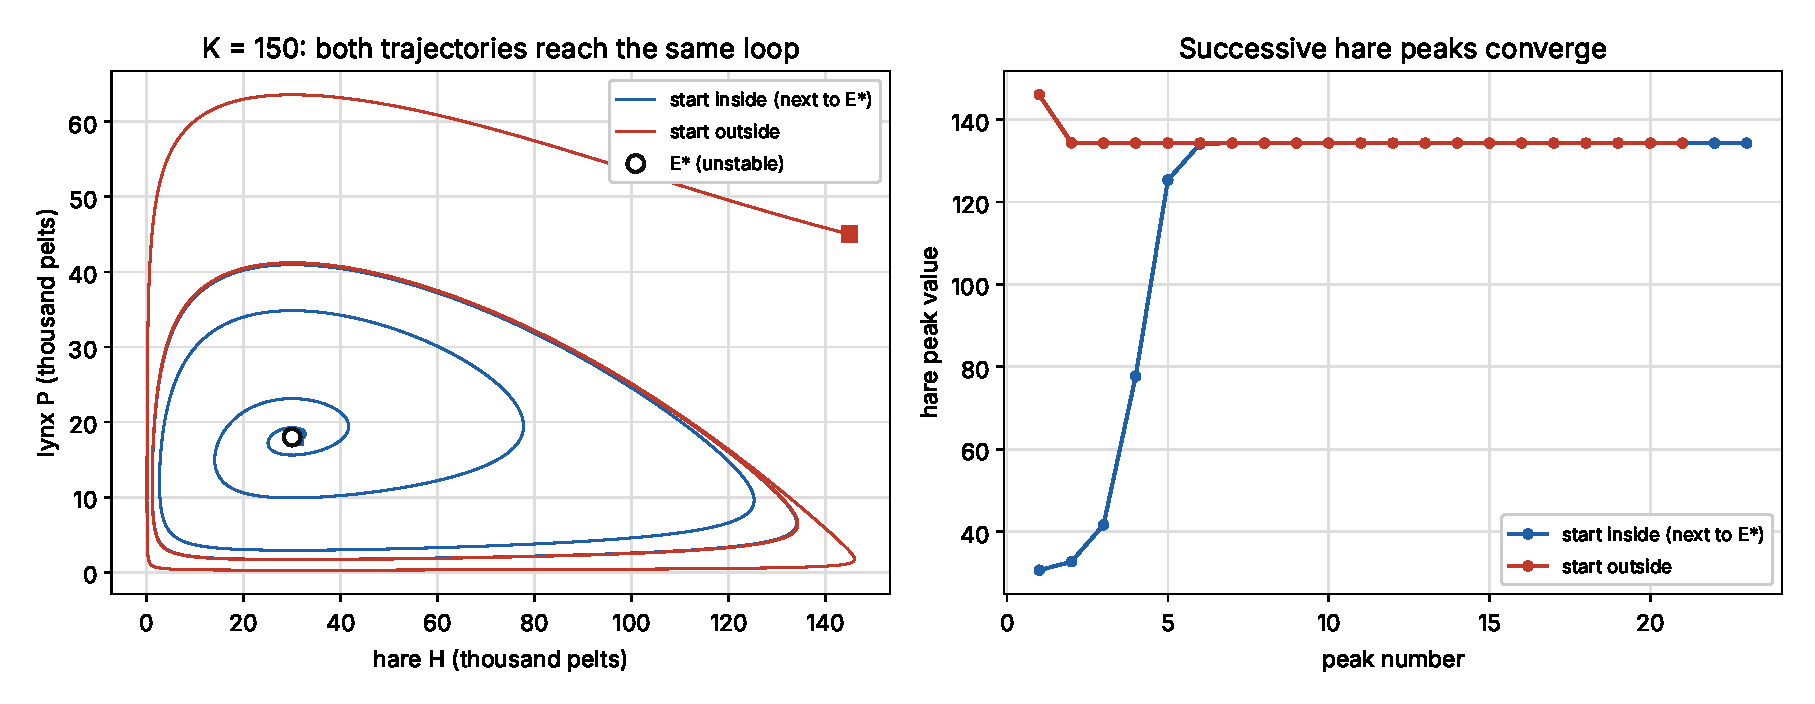
\includegraphics[width=0.9\linewidth]{rishi_limit_cycle}
  \caption{At $K=150$, trajectories started inside and outside the cycle converge onto the same
  closed orbit (left); their successive hare maxima approach a common value (right).}
  \label{fig:rishi_cycle}
\end{figure}

\subsection{Bifurcation in $K$}

Root-finding on the numerically evaluated trace of $J(E^*)$ places the sign change at
$K=90.0000000000$, in agreement with $K_H=b+2H^*$ and Figure~\ref{fig:trace-det}; there the
eigenvalues are $\pm0.632i=\pm i\omega_0$, and they become complex (node to focus) at $K\approx42.6$.

The numerical bifurcation diagram (Figure~\ref{fig:rishi_bif}) records the post-transient maximum
and minimum for 113 values of $K$ between 32 and 200. For $K<89$ the two coincide (largest
spread $5\times10^{-5}$): the solution settles on $E^*$. At $K_H$ the branches separate continuously
from the equilibrium and the cycle grows with $K$. Just above the threshold its half-amplitude
follows $A\approx7.8\sqrt{K-K_H}$, with fitted log--log slope $0.507$ for $0.5\le K-K_H\le8$
(Figure~\ref{fig:rishi_amp}), and the period approaches $T_0=9.93$ years ($9.97$ years at
$K-K_H=0.5$). This square-root growth from zero amplitude is the signature of a supercritical
Hopf bifurcation, consistent with the negative first Lyapunov coefficient of
Section~\ref{sec:joel}. As $K$ increases further the cycle minima approach zero: at $K=200$ the
hare minimum is $0.12$ thousand pelts, the paradox of enrichment~\cite{rosenzweig1971}.

\begin{figure}[htbp]
  \centering
  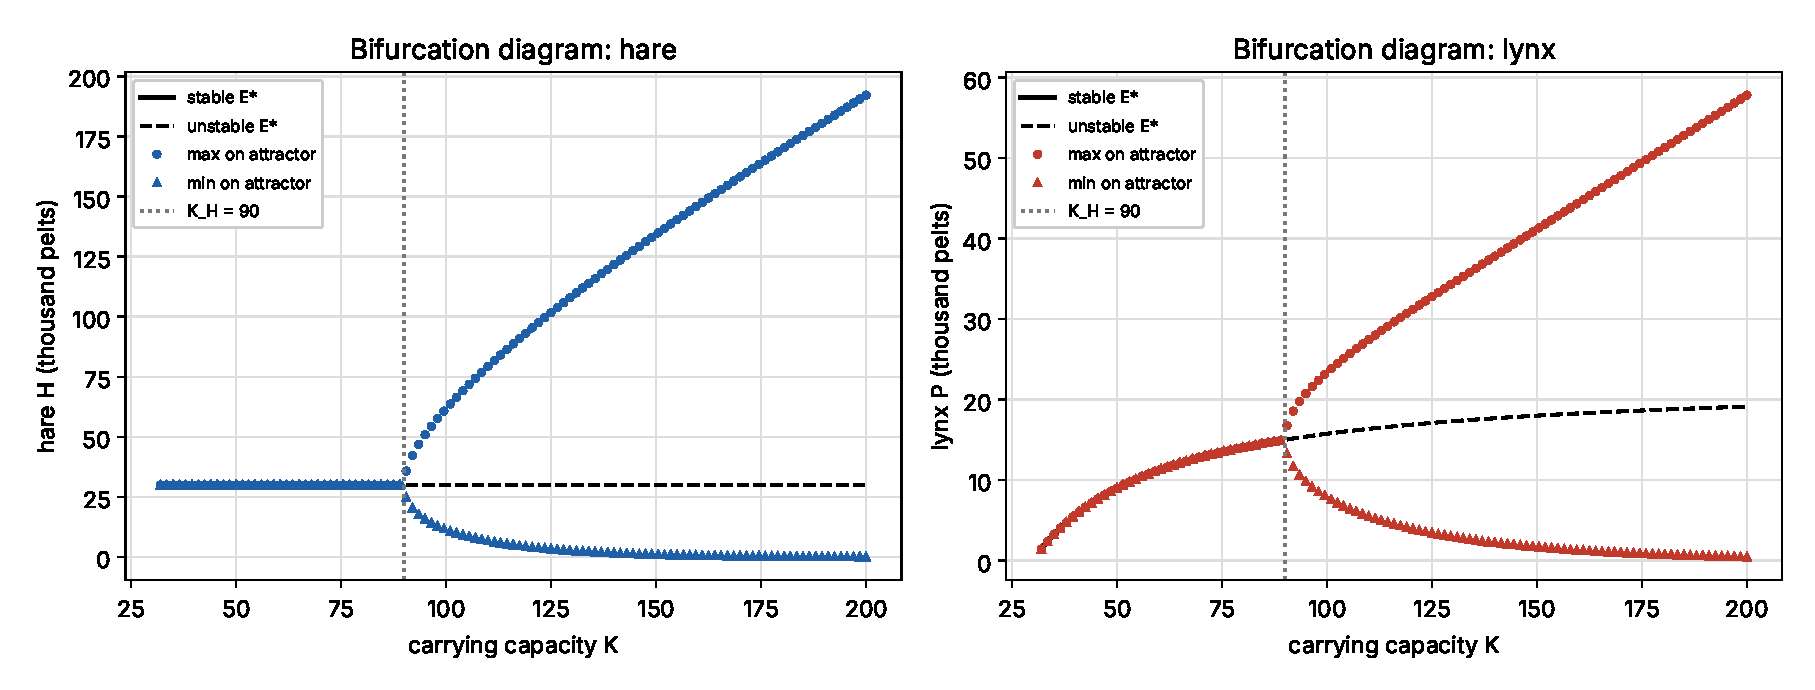
\includegraphics[width=0.9\linewidth]{rishi_bifurcation}
  \caption{Numerical bifurcation diagram: maximum and minimum of $H$ (left) and $P$ (right) after
  the burn-in, against $K$. Solid/dashed black: stable/unstable $E^*$. A cycle is born at
  $K_H=90$ with zero amplitude and its minima approach zero as $K$ grows.}
  \label{fig:rishi_bif}
\end{figure}

\begin{figure}[htbp]
  \centering
  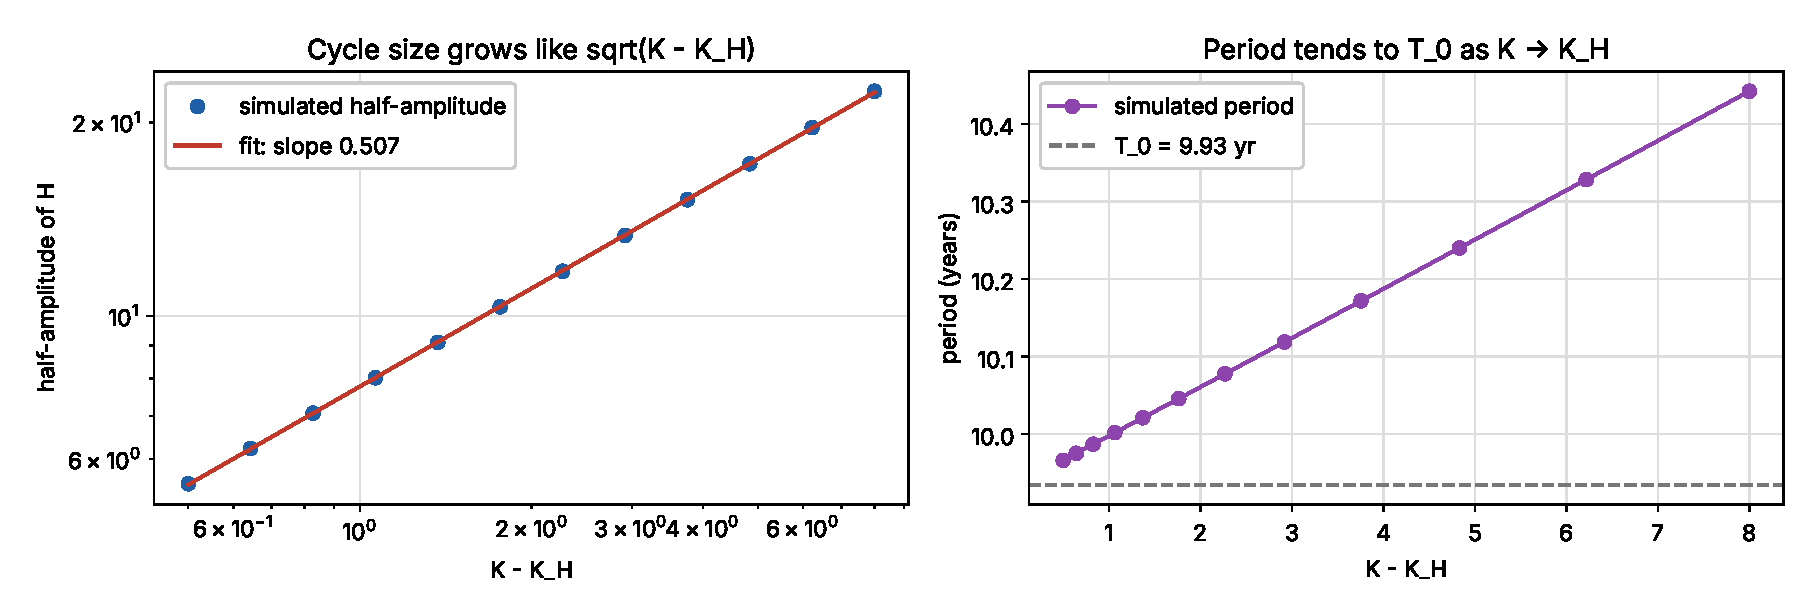
\includegraphics[width=0.9\linewidth]{rishi_amplitude_period}
  \caption{Left: half-amplitude of $H$ against $K-K_H$ on log--log axes, with slope $0.507$
  (supercritical prediction $1/2$). Right: cycle period, tending to $T_0=2\pi/\omega_0$.}
  \label{fig:rishi_amp}
\end{figure}

\subsection{Scope}

These simulations use illustrative, unfitted parameters and provide numerical evidence for one
parameter set, not proofs. Near $K_H$ the results depend on the burn-in length, which is why it
is lengthened there. Whether the historical hare--lynx series lies above or below the threshold
depends on $\sigma=K/K_H$ at the fitted parameters and is addressed in the fitting sections.
   (standalone build: rishi_main.tex)
%  Needs: amsmath, amssymb, booktabs, graphicx (PDF companions are used under pdflatex)
%  Figures: graphs/rishi_*.{eps,pdf}
%  Regenerate: python scripts/rishi_simulations.py   (numbers: results/simulations/)
%              python scripts/rishi_historical_placement.py   (results/simulations/historical/)
%  Code: src/lynx_hare/simulation.py, src/lynx_hare/simulation_plots.py,
%        notebooks/rishi_simulations.ipynb
% =====================================================================

\section{Numerical Simulations}\label{sec:rishi}

Section~\ref{sec:joel} locates the Hopf threshold $K_H=b+2H^*$ analytically. Linearisation is,
however, a local statement about the equilibrium at a single parameter value. This section tests
those predictions numerically and measures what linear analysis cannot give: the long-run
behaviour away from $E^*$, the size and period of the cycle, and the shape of the bifurcation.
Every trajectory is computed with the group's shared right-hand side of~\eqref{eq:rm}.

\subsection{Method}

\paragraph{Parameters.} We use the illustrative, unfitted values of Section~\ref{sec:joel}:
$r=1.5$, $a=4$, $b=30$, $e=0.4$, $m=0.8$ ($H,P$ in thousands of pelts, $t$ in years), for which
$H^*=30$, $K_H=90$ and $T_0=2\pi/\omega_0\approx 9.94$ years. The carrying capacity $K$ is varied.

\paragraph{Solver.} Equations~\eqref{eq:rm} are integrated with the adaptive Dormand--Prince
Runge--Kutta pair (RK45) in \texttt{scipy.integrate.solve\_ivp}~\cite{dormand1980,scipysolve}.
At each step a fourth- and a fifth-order estimate are formed from the same seven slope
evaluations; their difference estimates the local error, and the step is rejected and reduced
whenever this exceeds $\texttt{rtol}\,|y|+\texttt{atol}$. The project uses two settings of this
solver for two different jobs. Fitting and the 1900--1920 forecasts of the historical sections use
\texttt{model.solve} with $\texttt{rtol}=10^{-8}$, $\texttt{atol}=10^{-10}$ and a maximum step of
$0.1$ years, identical for both fitting methods. The long-run simulations in this section run for
thousands of years, so they use tighter tolerances, $\texttt{rtol}=10^{-10}$ and
$\texttt{atol}=10^{-12}$, without a step cap. Both call the same shared right-hand side. The
illustrative runs start from $(H_0,P_0)=(20,5)$; all values are in
\texttt{configs/simulations.json}.

\paragraph{Long-run behaviour.} To describe the attractor we integrate for a burn-in period
$T_{\mathrm{burn}}$, discard it, and record the next 300--400 years. On the recorded window we
report the range of $H$ and $P$; if $H$ still oscillates, the period is the mean interval between
successive hare maxima and the lag is the mean delay from a hare maximum to the next lynx
maximum. We take $T_{\mathrm{burn}}=3000$ years, increased to $20{,}000$ years when
$|K-K_H|<1$, where the equilibrium is a weak focus and transients decay very slowly.

\subsection{Solver accuracy}

The classical Lotka--Volterra system $\dot H=\alpha H-\beta HP$, $\dot P=\delta HP-\gamma P$
conserves $V=\delta H-\gamma\ln H+\beta P-\alpha\ln P$, so any drift in $V$ along a computed
orbit is numerical error. Over 100 time units RK45 keeps $|V(t)-V(0)|$ below $4\times10^{-10}$,
whereas explicit Euler with step $h=0.01$ drifts by $0.15$ and its orbit spirals outward
(Figure~\ref{fig:rishi_solver}), creating oscillatory growth the model does not have. For
Rosenzweig--MacArthur at $K=150$, tightening both tolerances a hundredfold changes the
solution by a relative $8\times10^{-10}$, and all states remain positive, as Lemma~\ref{lem:bounded}
requires.

\begin{figure}[htbp]
  \centering
  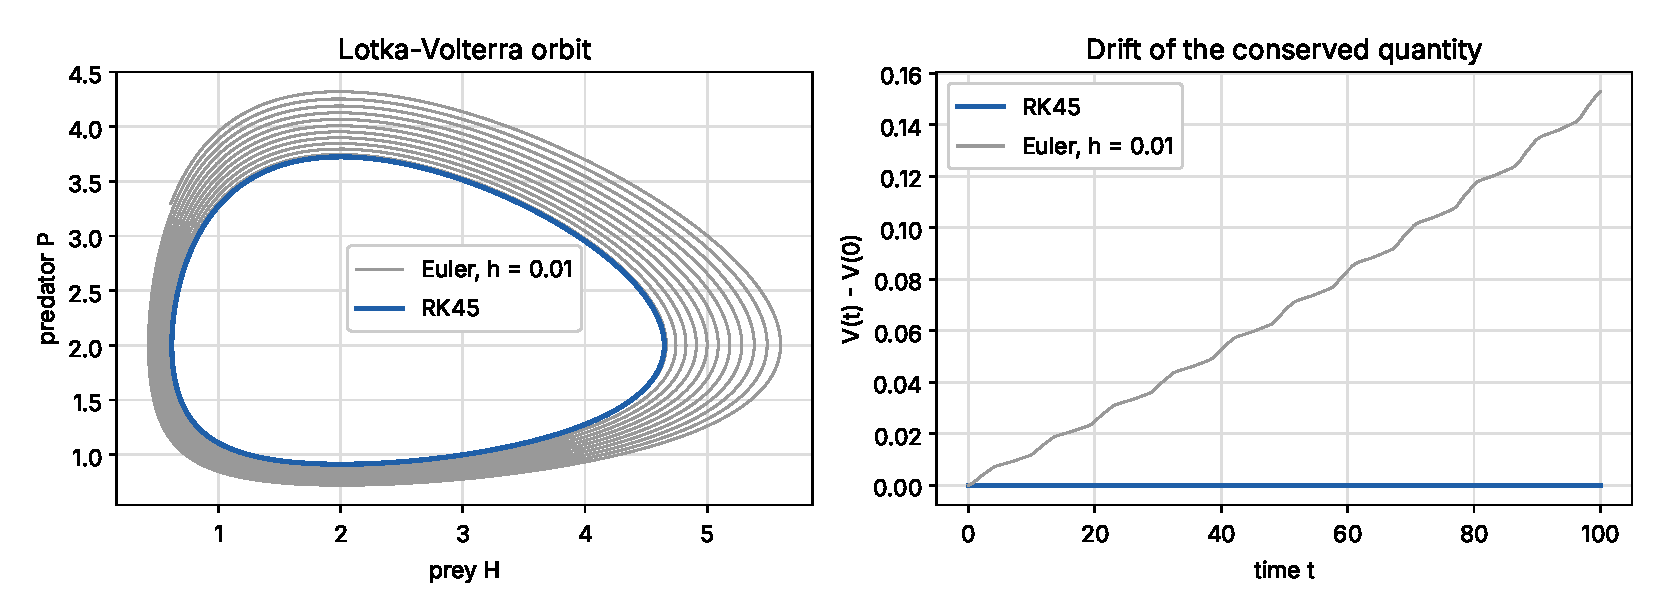
\includegraphics[width=0.9\linewidth]{rishi_solver_validation}
  \caption{Solver check on Lotka--Volterra. RK45 preserves the conserved quantity $V$ and
  closes the orbit; Euler ($h=0.01$) drifts and spirals outward. Only an accurate solver can
  distinguish a genuine limit cycle from a numerical artefact.}
  \label{fig:rishi_solver}
\end{figure}

\subsection{Reproduction of the analytic regimes}

Table~\ref{tab:rishi_regimes} reproduces each validation target of Section~\ref{sec:joel}
(3000-year burn-in throughout). Regime~D lies exactly on $K_H$: the residual oscillation there is
a slowly decaying transient (decay is only algebraic at a weak focus), not a cycle.

\begin{table}[htbp]
  \centering
  \caption{Simulated long-run behaviour for the regimes of Section~\ref{sec:joel}. Ranges are
  over 400 years after the burn-in; period and lynx lag are in years.}
  \label{tab:rishi_regimes}
  \begin{tabular}{clccccc}
    \toprule
    & $K$ & Eigenvalues & $H$ range & $P$ range & Period & Lag \\
    \midrule
    A & 25  & $-1.5,\ -0.073$ ($E_1$) & $25.0$         & $0$              & -- & -- \\
    B & 60  & $-0.188\pm0.515i$ & $30.0$         & $11.25$          & -- & -- \\
    C & 85  & $-0.022\pm0.623i$ & $30.0$         & $14.56$          & -- & -- \\
    D & 90  & $\pm0.632i$       & $[28.5,31.6]$  & $[14.51,15.49]$  & 9.94  & 2.50 \\
    E & 95  & $+0.020\pm0.640i$ & $[15.8,50.9]$  & $[9.81,20.75]$   & 10.25 & 2.81 \\
    F & 150 & $+0.150\pm0.676i$ & $[1.1,134.3]$  & $[1.69,41.16]$   & 13.91 & 4.52 \\
    \bottomrule
  \end{tabular}
\end{table}

Figure~\ref{fig:rishi_regimes} shows four of these regimes. Below the threshold (B, C) the
predator nullcline meets the prey hump to the right of its peak and trajectories spiral into
$E^*$; at $K=85$ the trace is only $-0.044$, so the decay takes centuries. Above the threshold
(E, F) the intersection lies left of the peak, $E^*$ repels, and the orbit settles onto a
sustained cycle that circulates counter-clockwise, with lynx peaks lagging hare peaks.

\begin{figure}[htbp]
  \centering
  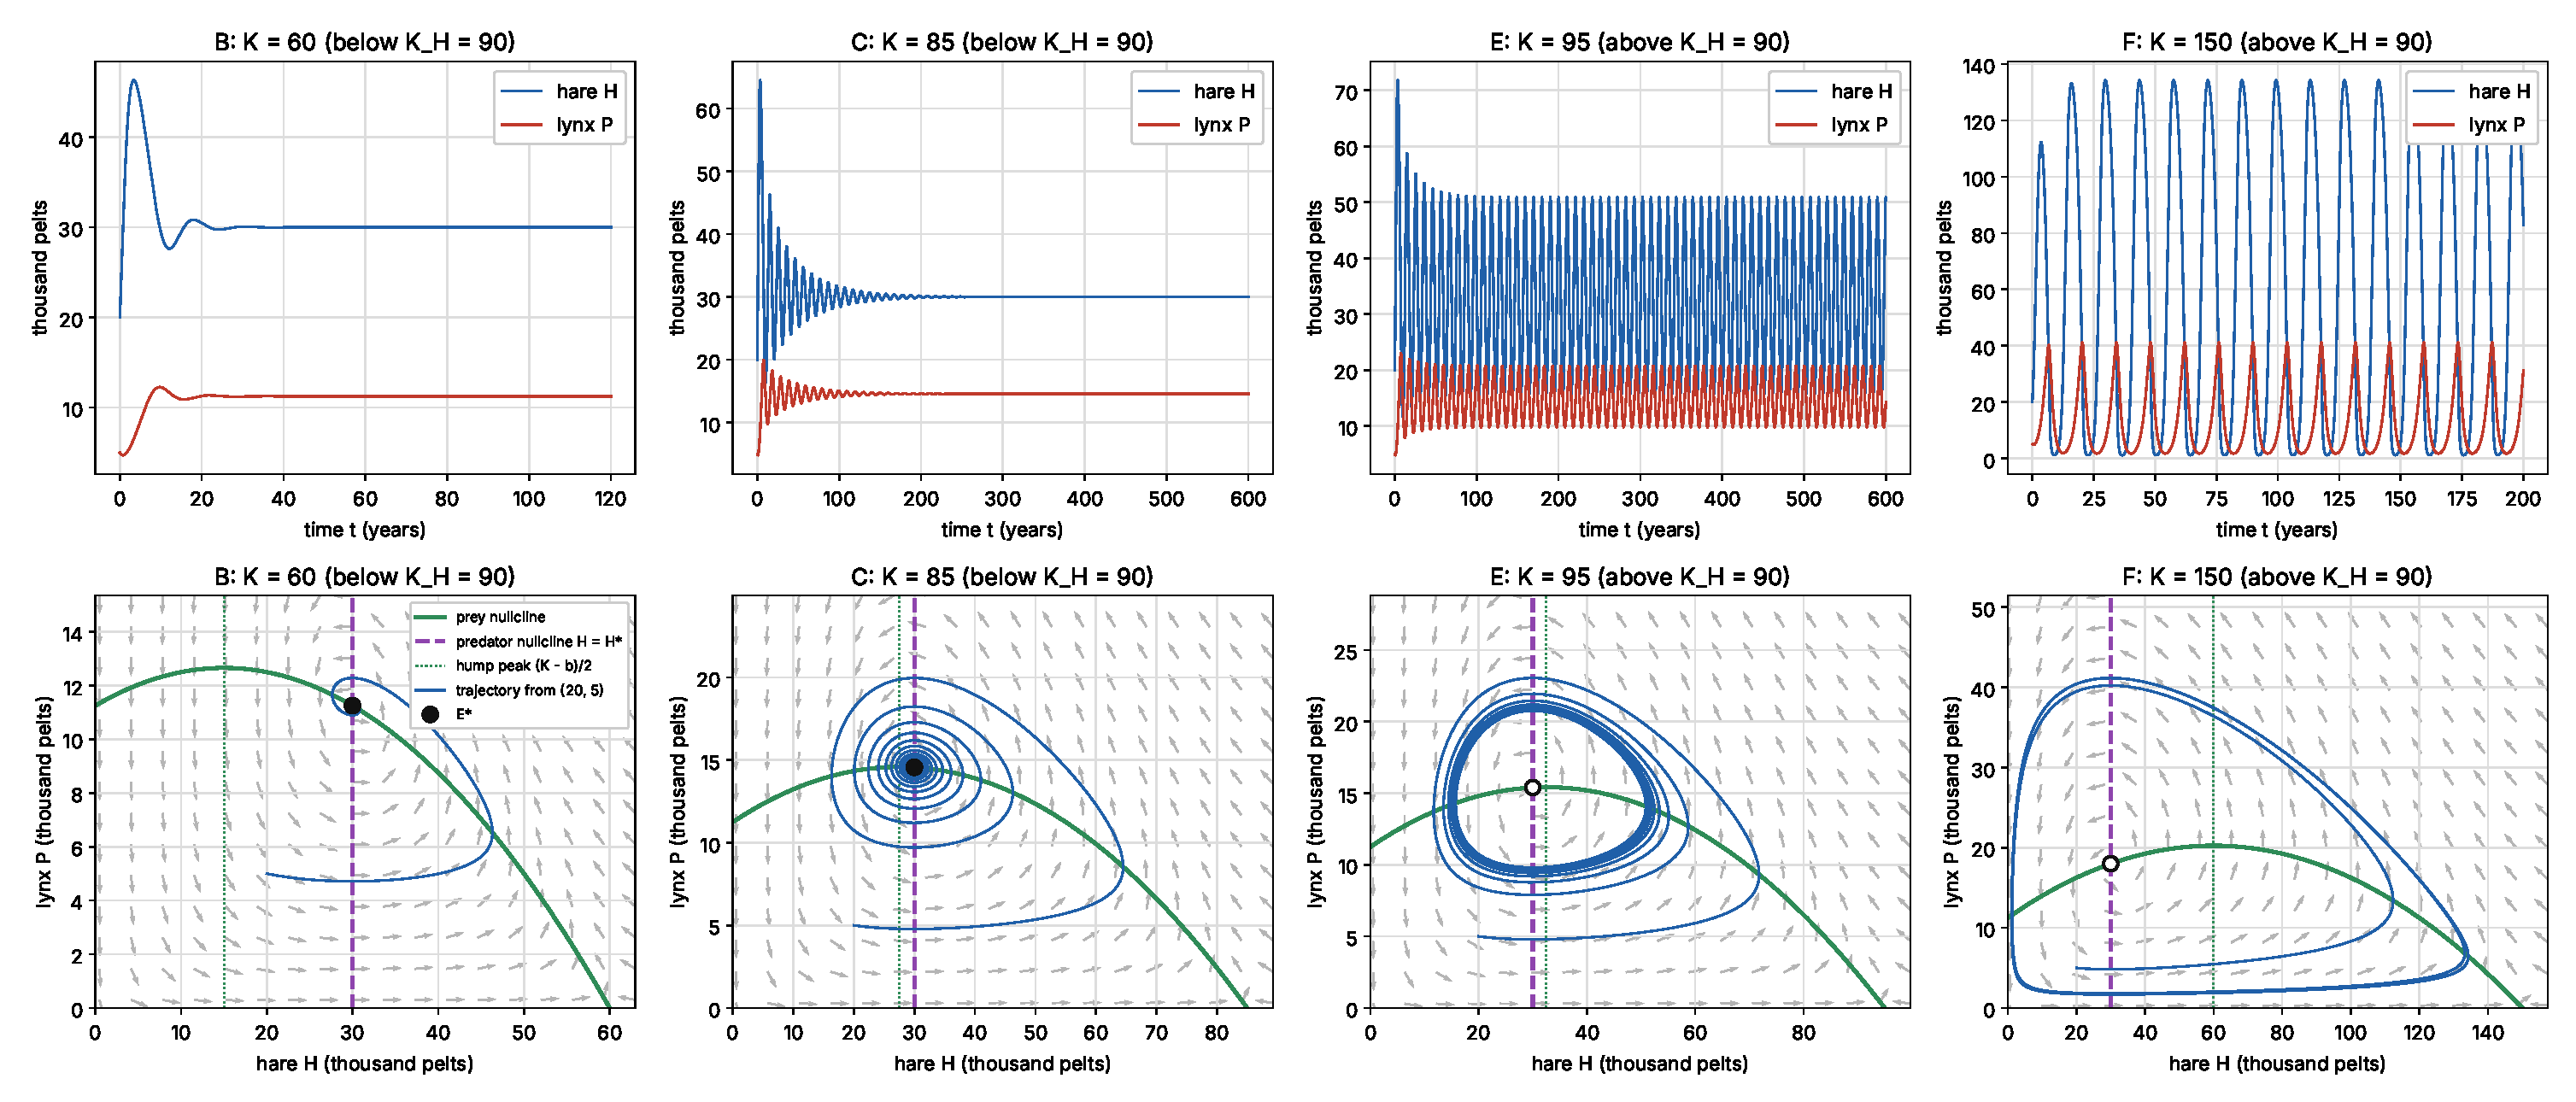
\includegraphics[width=\linewidth]{rishi_regimes}
  \caption{Time series (top) and phase portraits (bottom) from $(20,5)$ for $K=60,85$ (below
  $K_H=90$) and $K=95,150$ (above). Green: prey nullcline; dashed purple: predator nullcline
  $H=H^*$; dotted: hump peak $(K-b)/2$. Filled/open circle: stable/unstable $E^*$. Oscillations
  decay below $K_H$ and persist above it.}
  \label{fig:rishi_regimes}
\end{figure}

\subsection{The limit cycle attracts}

For Lotka--Volterra every initial condition lies on its own closed orbit. At $K=150$ we start one
trajectory beside the unstable equilibrium and one far outside the cycle
(Figure~\ref{fig:rishi_cycle}). The first spirals outward, the second inward, and their successive
hare maxima converge to the same value, $134.277$. The cycle is therefore orbitally stable,
in agreement with the uniqueness result cited in Section~\ref{sec:joel}~\cite{cheng1981}.

\begin{figure}[htbp]
  \centering
  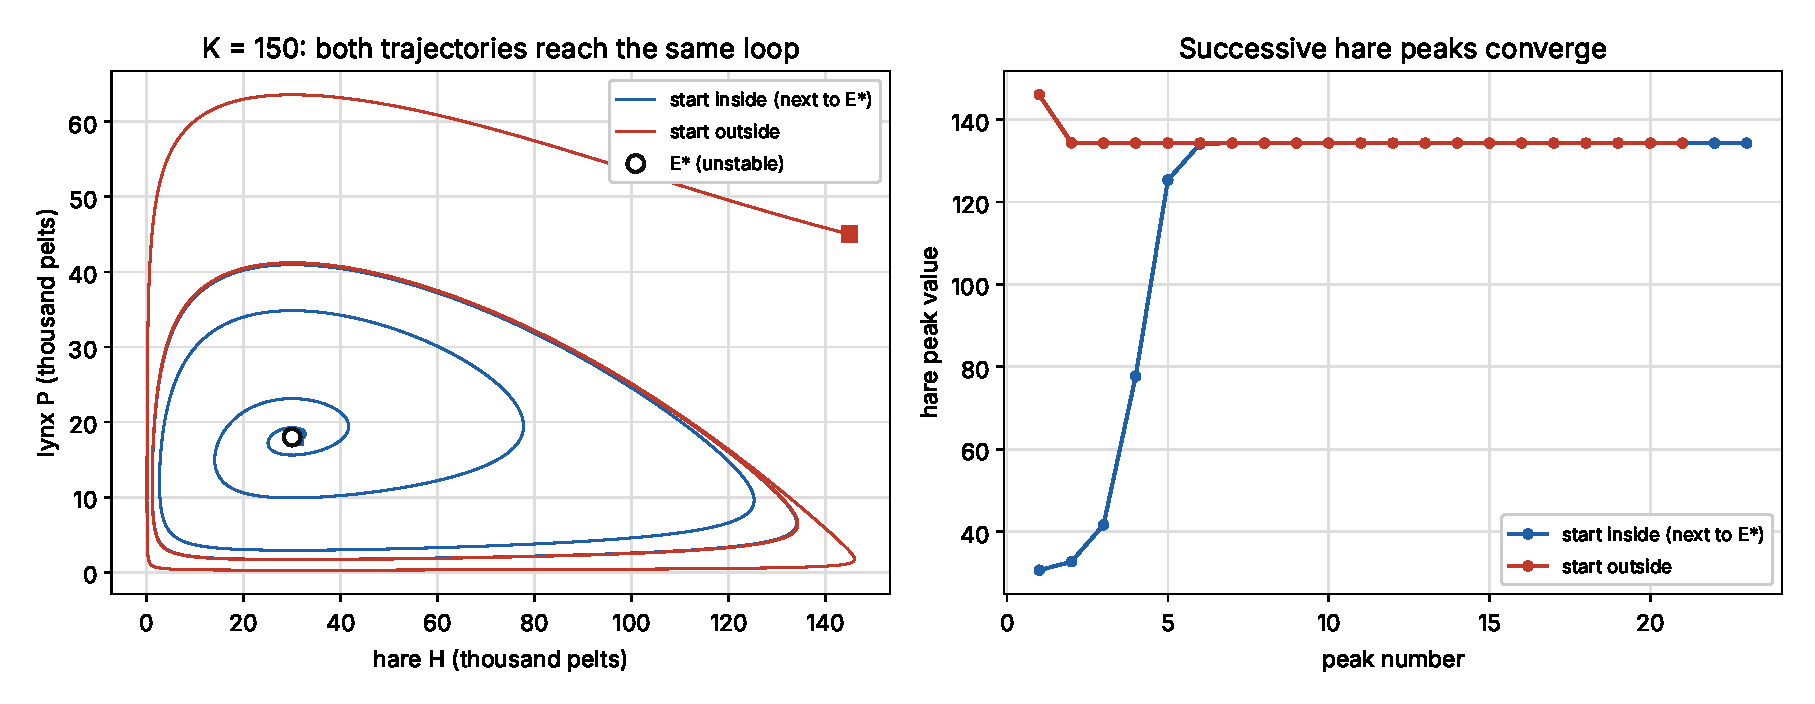
\includegraphics[width=0.9\linewidth]{rishi_limit_cycle}
  \caption{At $K=150$, trajectories started inside and outside the cycle converge onto the same
  closed orbit (left); their successive hare maxima approach a common value (right).}
  \label{fig:rishi_cycle}
\end{figure}

\subsection{Bifurcation in $K$}

Root-finding on the numerically evaluated trace of $J(E^*)$ places the sign change at
$K=90.0000000000$, in agreement with $K_H=b+2H^*$ and Figure~\ref{fig:trace-det}; there the
eigenvalues are $\pm0.632i=\pm i\omega_0$, and they become complex (node to focus) at $K\approx42.6$.

The numerical bifurcation diagram (Figure~\ref{fig:rishi_bif}) records the post-transient maximum
and minimum for 113 values of $K$ between 32 and 200. For $K<89$ the two coincide (largest
spread $5\times10^{-5}$): the solution settles on $E^*$. At $K_H$ the branches separate continuously
from the equilibrium and the cycle grows with $K$. Just above the threshold its half-amplitude
follows $A\approx7.8\sqrt{K-K_H}$, with fitted log--log slope $0.507$ for $0.5\le K-K_H\le8$
(Figure~\ref{fig:rishi_amp}), and the period approaches $T_0=9.93$ years ($9.97$ years at
$K-K_H=0.5$). This square-root growth from zero amplitude is the signature of a supercritical
Hopf bifurcation, consistent with the negative first Lyapunov coefficient of
Section~\ref{sec:joel}. As $K$ increases further the cycle minima approach zero: at $K=200$ the
hare minimum is $0.12$ thousand pelts, the paradox of enrichment~\cite{rosenzweig1971}.

\begin{figure}[htbp]
  \centering
  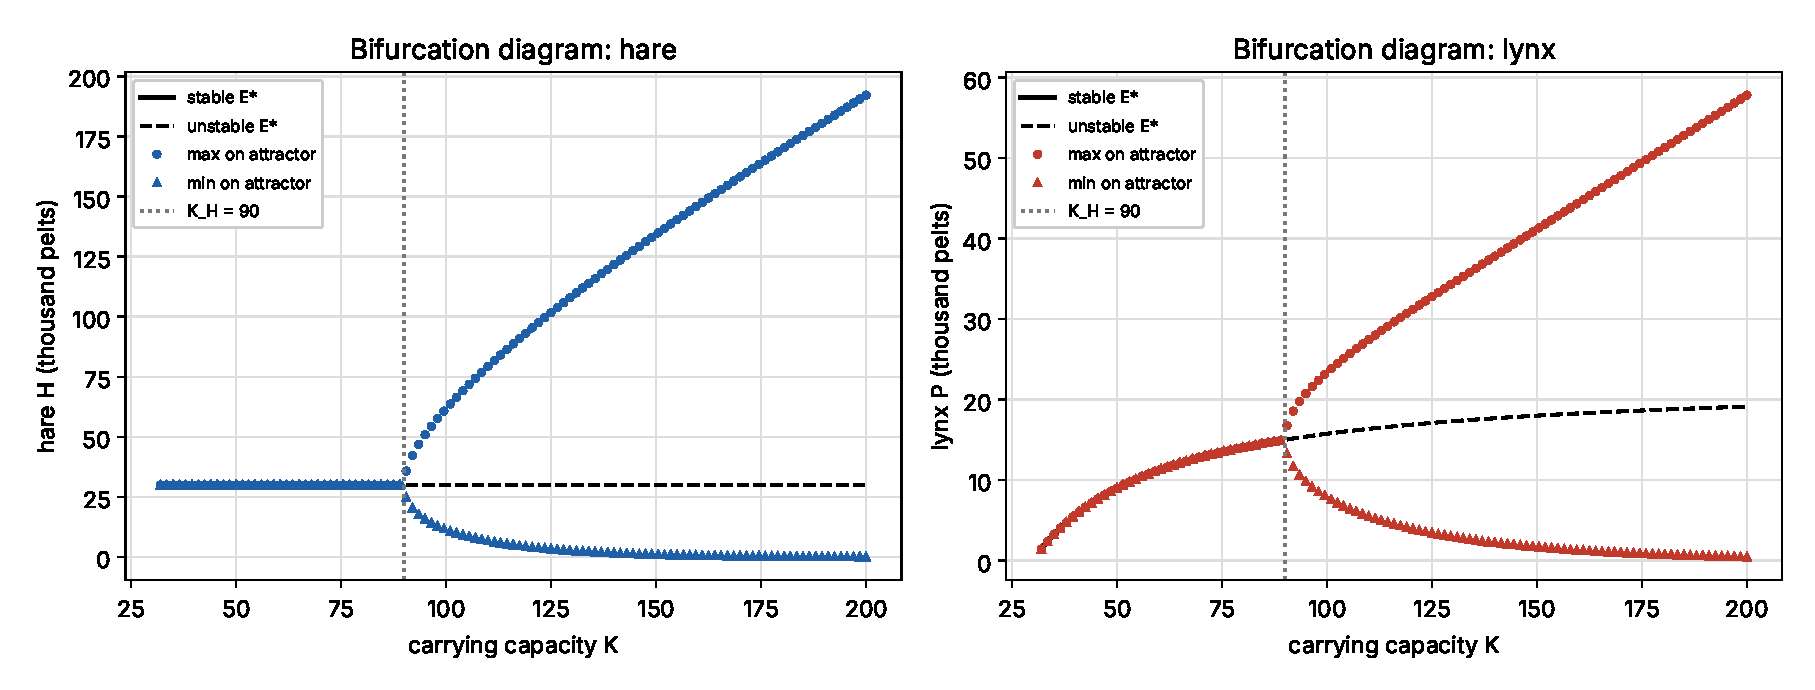
\includegraphics[width=0.9\linewidth]{rishi_bifurcation}
  \caption{Numerical bifurcation diagram: maximum and minimum of $H$ (left) and $P$ (right) after
  the burn-in, against $K$. Solid/dashed black: stable/unstable $E^*$. A cycle is born at
  $K_H=90$ with zero amplitude and its minima approach zero as $K$ grows.}
  \label{fig:rishi_bif}
\end{figure}

\begin{figure}[htbp]
  \centering
  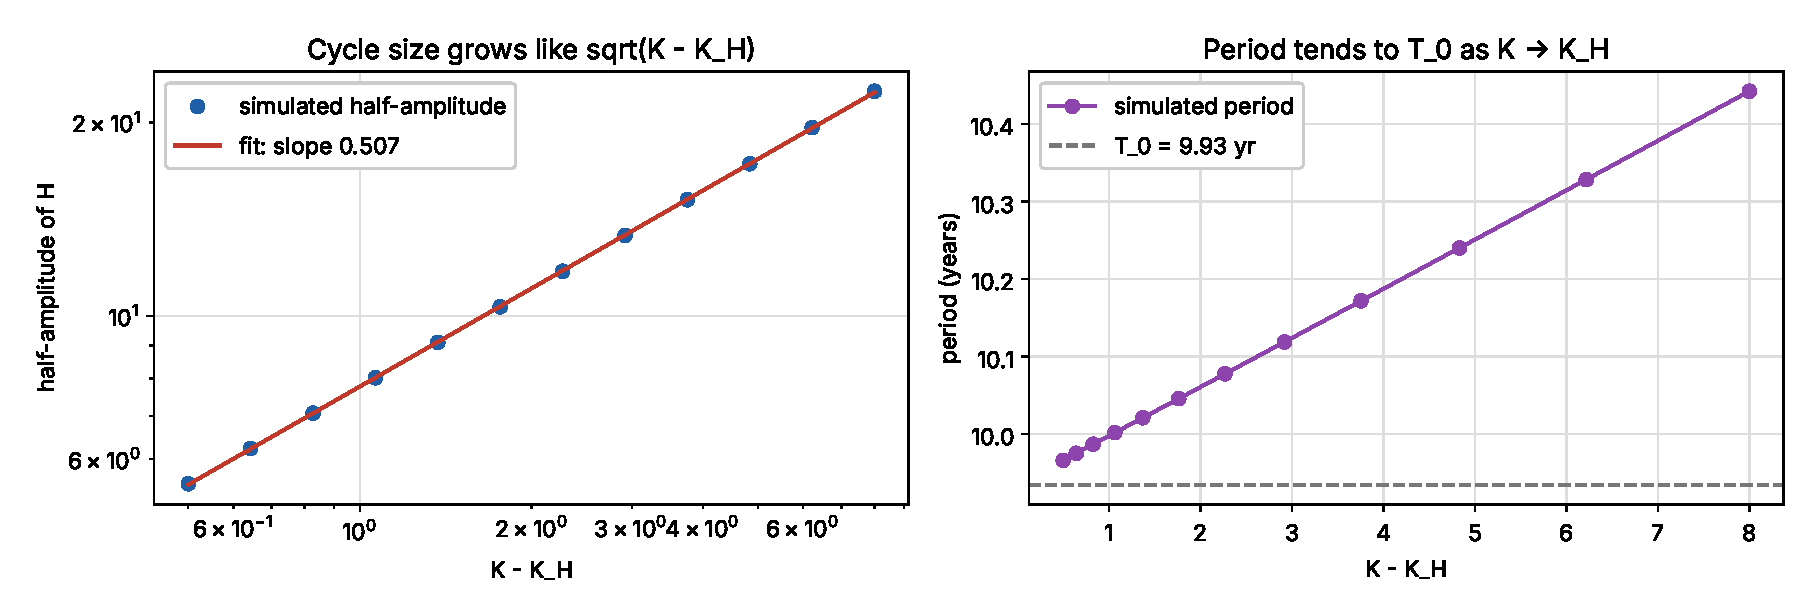
\includegraphics[width=0.9\linewidth]{rishi_amplitude_period}
  \caption{Left: half-amplitude of $H$ against $K-K_H$ on log--log axes, with slope $0.507$
  (supercritical prediction $1/2$). Right: cycle period, tending to $T_0=2\pi/\omega_0$.}
  \label{fig:rishi_amp}
\end{figure}

\subsection{Scope}

These simulations use illustrative, unfitted parameters and provide numerical evidence for one
parameter set, not proofs. Near $K_H$ the results depend on the burn-in length, which is why it
is lengthened there. Whether the historical hare--lynx series lies above or below the threshold
depends on $\sigma=K/K_H$ at the fitted parameters and is addressed in the fitting sections.
